\documentclass[11pt,oneside]{article}
\usepackage[T1]{fontenc}
\usepackage[utf8]{inputenc}
%\DeclareUnicodeCharacter{00A0}{ }
\usepackage[adobe-utopia]{mathdesign}

\usepackage{amsmath}
\usepackage[francais]{babel}
\usepackage[dvips]{graphicx}
%\usepackage{here}
\usepackage{framed}
\usepackage[normalem]{ulem}
\usepackage{fancyhdr}
\usepackage{titlesec}
\usepackage{vmargin}

\usepackage{amsmath}
\usepackage{ifthen}
\usepackage{multirow}
\usepackage{multicol} % Portions de texte en colonnes

%\usepackage{xltxtra} % Logo XeLaTeX
%\usepackage{pst-solides3d}
\usepackage{color}
%\usepackage{colortbl}
\usepackage{titletoc} % Pour la mise en forme de la table des matières

%\usepackage[crop=off]{auto-pst-pdf}
%\usepackage{bclogo}


%\usepackage{longtable}
%\usepackage{flafter}%floatants après la référence
%\usepackage{pst-solides3d}
%\usepackage{pstricks}
%\usepackage{minitoc}
%\setcounter{minitocdepth}{4}
%\usepackage{draftcopy}% "Brouillon"
%\usepackage{floatflt}
%\usepackage{psfrag}
%\usepackage{listings} % Permet d'insérer du code de programmation
%\usepackage{lmodern}
%\usepackage[adobe-utopia,uppercase=upright,greeklowercase=upright]{mathdesign}
%\usepackage{minionpro}
%\usepackage{pifont}
%\usepackage{amssymb}
%\usepackage[francais]{varioref}

\setmarginsrb{1.5cm}{1cm}{1cm}{1.5cm}{1cm}{1cm}{1cm}{1cm}

\definecolor{gris25}{gray}{0.75}
\definecolor{bleu}{RGB}{18,33,98}
\definecolor{bleuf}{RGB}{42,94,171}
\definecolor{bleuc}{RGB}{231,239,247}
\definecolor{rougef}{RGB}{185,18,27}
\definecolor{rougec}{RGB}{255,230,231}
\definecolor{vertf}{RGB}{103,126,82}
\definecolor{vertc}{RGB}{220,255,191}
\definecolor{violetf}{RGB}{112,48,160}
\definecolor{violetc}{RGB}{230,224,236}
\definecolor{jaunec}{RGB}{220,255,191}
\usepackage[raccourcis]{FAST}
\usepackage[%
    pdftitle={IS -- Introduction},
    pdfauthor={Xavier Pessoles},
    colorlinks=true,
    linkcolor=blue,
    citecolor=magenta]{hyperref}

\usepackage{pifont}


% \makeatletter \let\ps@plain\ps@empty \makeatother
%% DEBUT DU DOCUMENT
%% =================
\sloppy
\hyphenpenalty 10000

\newcommand{\Pointilles}[1][3]{%
\multido{}{#1}{\makebox[\linewidth]{\dotfill}\\[\parskip]
}}


\colorlet{shadecolor}{orange!15}

\newtheorem{theorem}{Theorem}


\begin{document}


\newboolean{prof}
\setboolean{prof}{true}
%------------- En tetes et Pieds de Pages ------------
\pagestyle{fancy}
\renewcommand{\headrulewidth}{0pt}

\fancyhead{}
\fancyhead[L]{%
\noindent\noindent\begin{minipage}[c]{2.6cm}
%Lycée Rouvière PTSI

\includegraphics[width=2cm]{png/logo_ptsi.png}%
\end{minipage}
}


\fancyhead[C]{\rule{12cm}{.5pt}}

\fancyhead[R]{%
\noindent\begin{minipage}[c]{3cm}
\begin{flushright}
\footnotesize{\textit{\textsf{Sciences Industrielles\\ de l'Ingénieur}}}%
\end{flushright}
\end{minipage}
}

\renewcommand{\footrulewidth}{0.2pt}

\fancyfoot[C]{\footnotesize{\bfseries \thepage}}
\fancyfoot[L]{\footnotesize{2013 -- 2014} \\ X. \textsc{Pessoles}}
\ifthenelse{\boolean{prof}}{%
\fancyfoot[R]{\footnotesize{Cours -- CI 1.01 : IS -- Introduction}}
}{%
\fancyfoot[R]{\footnotesize{Cours -- CI 6 : PPM}}
}



\begin{center}
 \huge\textsc{CI 1 -- IS}

 \large\textsc{Étude des systèmes pluritechniques et multiphysiques -- Initiation à l'Ingénierie Système}
\end{center}

\begin{center}
 \LARGE\textsc{Chapitre 1 -- Introduction à l'Ingénierie Systèmes}
\end{center}

%\begin{flushright}
%\textit{D'après documents de Jean-Pierre Pupier}
%\end{flushright}

\vspace{.5cm}


%\begin{minipage}[c]{.23\linewidth}
%\begin{center}
%\includegraphics[height=2.5cm]{png/tour_bois}
%
%\textit{Tour à bois \cite{tab}}
%\end{center}
%\end{minipage} \hfill
%\begin{minipage}[c]{.23\linewidth}
%\begin{center}
%\includegraphics[height=2.5cm]{png/cazeneuve}
%
%\textit{Tour conventionnel \cite{cazeneuve}}
%\end{center}
%\end{minipage} \hfill
%\begin{minipage}[c]{.23\linewidth}
%\begin{center}
%\includegraphics[height=2.5cm]{png/tour_mazak}
%
%\textit{Tour à commande numérique \cite{mazak}}
%\end{center}
%\end{minipage}\hfill
%\begin{minipage}[c]{.23\linewidth}
%\begin{center}
%\includegraphics[height=2.5cm]{png/plaquettes}
%
%\textit{Plaquettes de tournage \cite{plaquettes}}
%\end{center}
%\end{minipage}
%
%\vspace{.5cm}
%
%\begin{center}
%\includegraphics[height=7cm]{png/cycleV}
%\end{center}

%\begin{center}
%\includegraphics[width=.9\textwidth]{png/cyclev.png}

%\textit{Cycle de conception d'un produit}
%\end{center}

%\begin{prob}
%\textsc{Problématique :}
%\begin{itemize}
%\item %Quelles sont les conditions fonctionnelles permettant le fonctionnement du système ?
%\item %Quelle est la chaîne de côte unidirectionnelle correspondant à une condition donnée ?
%\end{itemize}
%\end{prob}



 
\noindent \begin{minipage}[c]{.55\linewidth}

\indent Quelles solutions utilisent les industriels pour proposer des produits compatibles avec le besoin des consommateurs ? Quelles solutions utilisent les industriels pour renouveler leur offre de produit ? Quelles solutions utilisent les industriels pour rester à la pointe de la technologie ? Quelles solutions utilisent les industriels pour mener à bien leurs projets ?

\end{minipage}
\begin{minipage}[c]{.4\linewidth}
\begin{center}
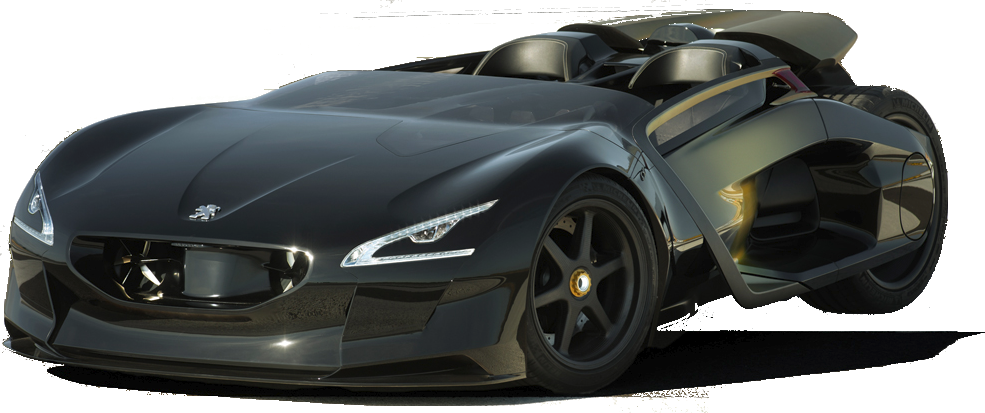
\includegraphics[width=.9\textwidth]{png/cc_ex1}

\textit{Concept car Peugeot Ex 1 \cite{cc_ex1} -- 100\% électrique}
\end{center}
\end{minipage}

\vspace{.5cm}

La bonne santé des industriels dépend de la réponse à ces questions. Pour cela de nombreux outils leurs permettent de maîtriser la conception, la réalisation, la diffusion et le recyclage des produits. 

Le but de l'Ingéniérie Système (IS) est de proposer des outils permettant d'aider les industriels lors de toute la vie d'un produit. 

\begin{prob}
Quels sont, dans un premier temps, les outils à notre disposition permettant de gérer au mieux la conception, la production, la diffusion et le recyclage des produits industriels ?
\end{prob}
\begin{savoir}
\textsc{Savoirs :}
\begin{itemize}
\item  A-C1.1 : Besoin, système, services attendus du système, cahier des charges fonctionnel, spécifications fonctionnelles, analyse du cycle de vie, acteurs, interactions, solution technique.
\begin{itemize}
\item A-C1.S1 : Décomposer une exigence en plusieurs exigences unitaires.
\item A-C1.S2 : Identifier les interactions entre les acteurs et le système étudié.
\end{itemize}
\item A-C3.1 : Analyse structurelle et comportementale.
\item A-C3.2 : Chaîne d'information, chaîne d'énergie.
\end{itemize}

\end{savoir}

\begin{center}
\url{http://xpessoles.ptsi.free.fr}

\url{xpessoles.ptsi@free.fr}

\end{center}

\setlength{\parskip}{0ex plus 0.2ex minus 0ex}
 \renewcommand{\contentsname}{}
 \renewcommand{\baselinestretch}{1}

\tableofcontents

 \renewcommand{\baselinestretch}{1.2}
\setlength{\parskip}{2ex plus 0.5ex minus 0.2ex}

% \vspace{1cm}
\textit{Ce document évolue. Merci de signaler toutes erreurs ou coquilles.}


\section{Définitions préliminaires}
\begin{defi}

\textbf{Produit} \cite{norme}

Résultat d'activité ou de processus.

\end{defi}
\begin{rem}
\begin{itemize}
\item Note 1 : le terme produit peut inclure les services, les matériels, les produits issus de processus à caractère continu, les logiciels ou une combinaison des deux.
\item Note 2 : un produit peut être matériel (par exemple, assemblages ou produits issus de processus à caractère continu) ou immatériel (par exemple, connaissances ou concepts), ou une combinaison des 2. 
\item Note 3 : un produit peut être soit intentionnel (par exemple une offre aux clients) soit non intentionnel (par exemple, un polluant ou des effets indésirables). 
\end{itemize}
\end{rem}



\begin{defi}
\textbf{Système}\cite{roques}\cite{debout}

Un système est un ensemble de composants interreliés qui interagissent les uns avec les autres d’une manière organisée pour accomplir une finalité commune (NASA 1995).

Un système est un ensemble intégré d’éléments qui accomplissent un objectif défini (INCOSE 2004)\footnotemark[1].

La frontière d’un système est une limite fictive qui permet d'isoler le système considéré et ses composants de son environnement (milieu extérieur).


\end{defi}
\footnotetext[1]{International Council on Systems Engineering}

\begin{rem}
On abordera régulièrement la notion de \textit{système complexe}. Un tel système est multiphysique et pluritechnologique. Cela signifie que son fonctionnement fait appel à plusieurs disciplines de la physique (mécanique, électronique, thermique, optique ...). Sa conception, sa fabrication et son fonctionnement font appel à un grand nombre de technologies. 
\end{rem}

\begin{exemple}

\noindent\begin{minipage}[c]{.22\linewidth}
\begin{center}
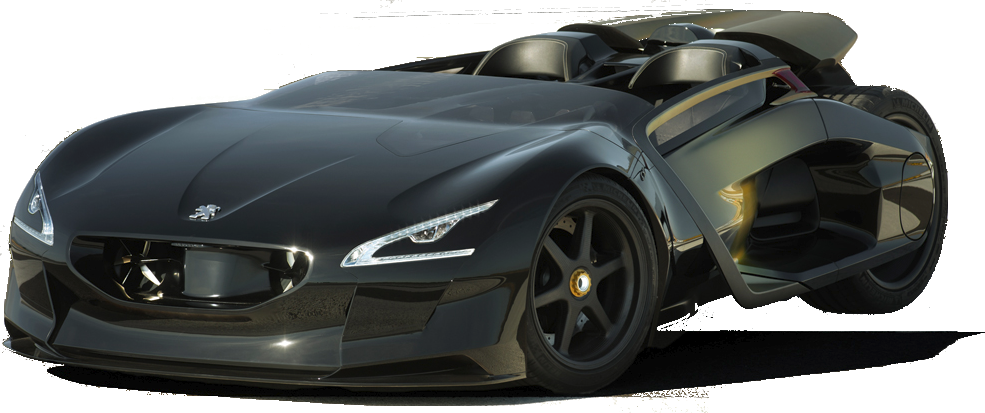
\includegraphics[width=\textwidth]{png/cc_ex1}

\textit{Automobile -- Concept car Peugeot EX1}
\end{center}
\end{minipage} \hfill
\begin{minipage}[c]{.22\linewidth}
\begin{center}
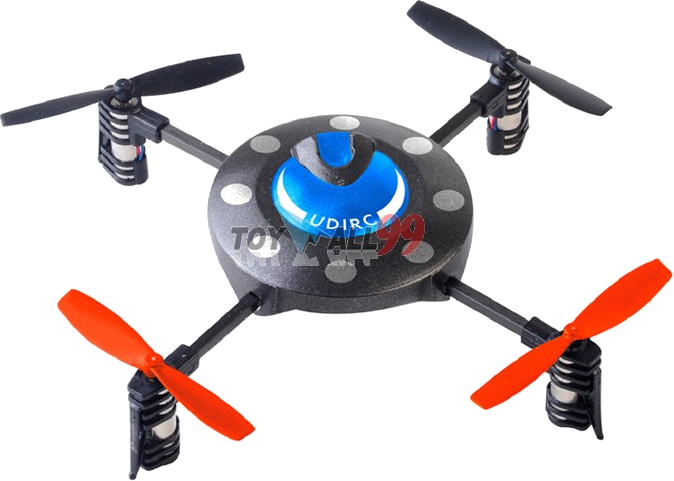
\includegraphics[width=.7\textwidth]{png/quadri}

\textit{Loisir -- Modélisme -- Drone quadrihélice}
\end{center}
\end{minipage} \hfill
\begin{minipage}[c]{.22\linewidth}
\begin{center}
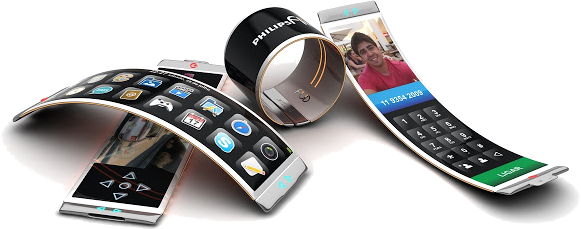
\includegraphics[width=\textwidth]{png/oled}

\textit{Électronique -- Téléphones à écrans flexilbes -- \textit{Oled} \cite{oled}}
\end{center}
\end{minipage}\hfill
\begin{minipage}[c]{.22\linewidth}
\begin{center}
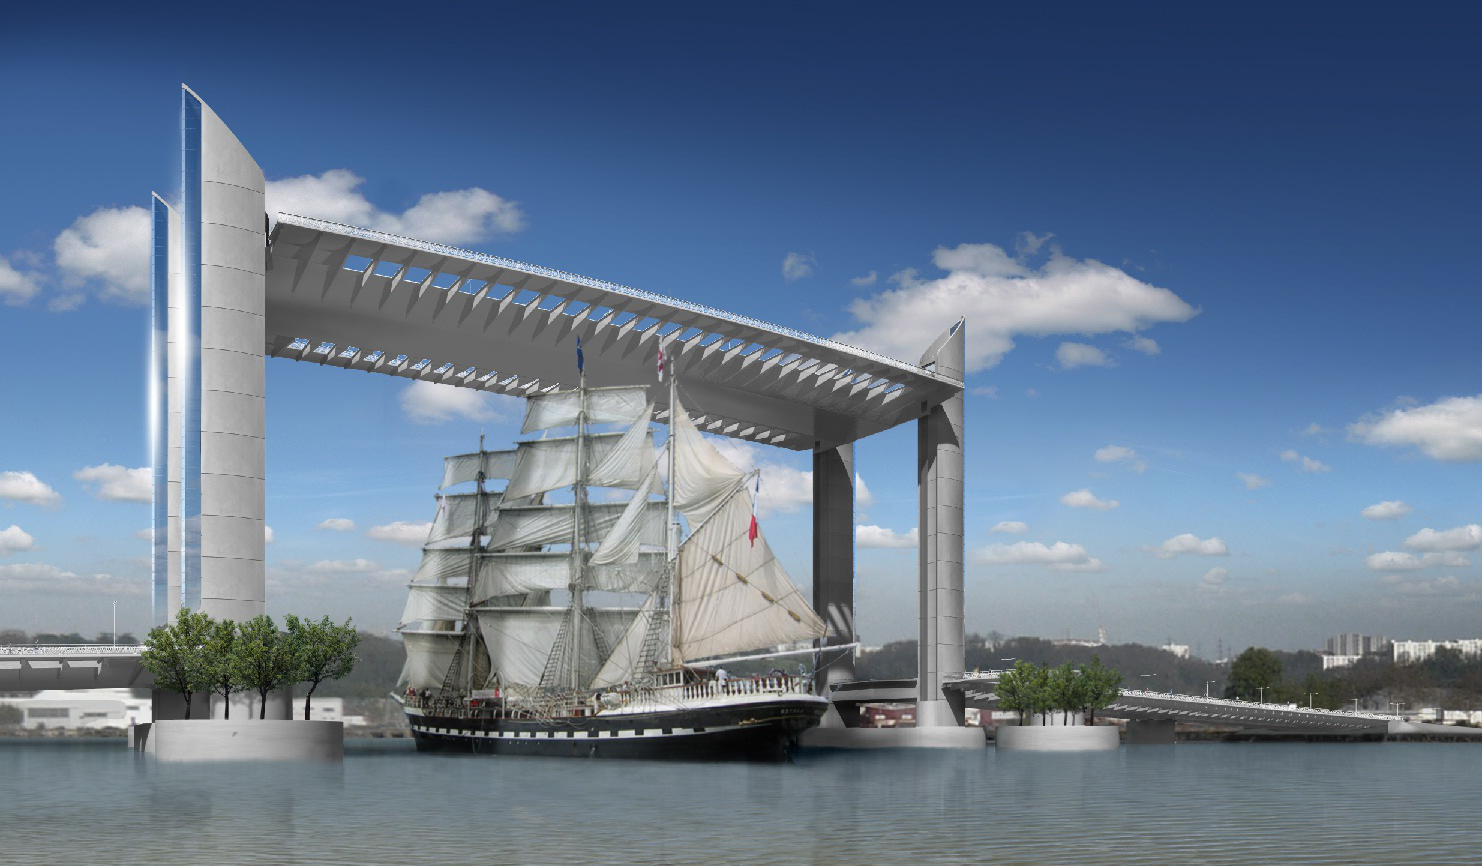
\includegraphics[width=\textwidth]{png/pont_bacalan}

\textit{Génie Civil -- Pont Bacalan Bordeaux\cite{pont}}
\end{center}
\end{minipage}

Ces systèmes sont multiphyiques et pluritechnologiques dans la mesure où ils intègrent à la fois de l'électronique ou de l'électrotechnique, de la mécanique, des matériaux innovants. 

\end{exemple}


\begin{defi}

\textbf{Utilisateur} \cite{norme}

Toute personne ou entité pour laquelle le produit est conçu et qui exploite au moins l'une de ses fonctions à un moment quelconque de son cycle de vie.


\textbf{Acteurs}\cite{roques}

Rôle joué par un utilisateur humain ou un autre système qui interagit directement avec le système étudié. Un acteur participe à au moins un cas d'utilisation.

\end{defi}

\begin{exemple}
\begin{itemize}
\item Acteur du concept car EX1 : conducteur du véhicule
\item Acteur du drone : joueur
\item Acteur du téléphone : utilisateur 
\item Acteur du pont : commandant de bord
\end{itemize}
\end{exemple}



\begin{defi}
\textbf{Interaction}

Une interaction avec un système complexe peut être défini par un échange d'un flux d'\textbf{énergie}, de \textbf{matière} ou d'\textbf{information}.
\end{defi}

\begin{exemple}
\begin{itemize}
\item Conducteur $\leftrightarrow$ Ex 1 : actions sur les commandes du véhicule entraînant son déplacement
\item Joueur $\leftrightarrow$ drone : action sur les commandes entraînant l'envol du drone
\item Utilisateur $\leftrightarrow$ téléphone : échange de voix
\item Commandant $\leftrightarrow$ pont : requêtes du commandant entraînant la levée ou la baissée du pont
\end{itemize}
\end{exemple}


\begin{defi}
\textbf{Besoin}\cite{norme}

Ce qui est nécessaire à l'utilisateur et désiré par lui.


C’est une exigence qui naît de la nature, de la vie sociale ou économique (Larousse). Le besoin ainsi défini concerne la nature des attentes de l'utilisateur et non le volume du marché.

\end{defi}

\begin{exemple}
\textit{J'ai besoin de me rendre au Mourillon.}

Plusieurs produits peuvent satisfaire le besoin du client. 

\noindent\begin{minipage}[c]{.22\linewidth}
\begin{center}
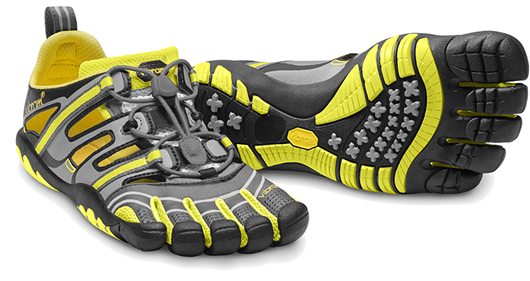
\includegraphics[width=\textwidth]{png/vibram}

\textit{Vibram fivefingers \cite{vibram}}
\end{center}
\end{minipage} \hfill
\begin{minipage}[c]{.22\linewidth}
\begin{center}
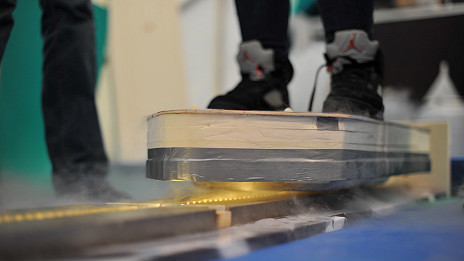
\includegraphics[width=.9\textwidth]{png/magsurf}

\textit{Magsurf -- Surf à sustentation magnétique \cite{magsurf}}
\end{center}
\end{minipage} \hfill
\begin{minipage}[c]{.22\linewidth}
\begin{center}
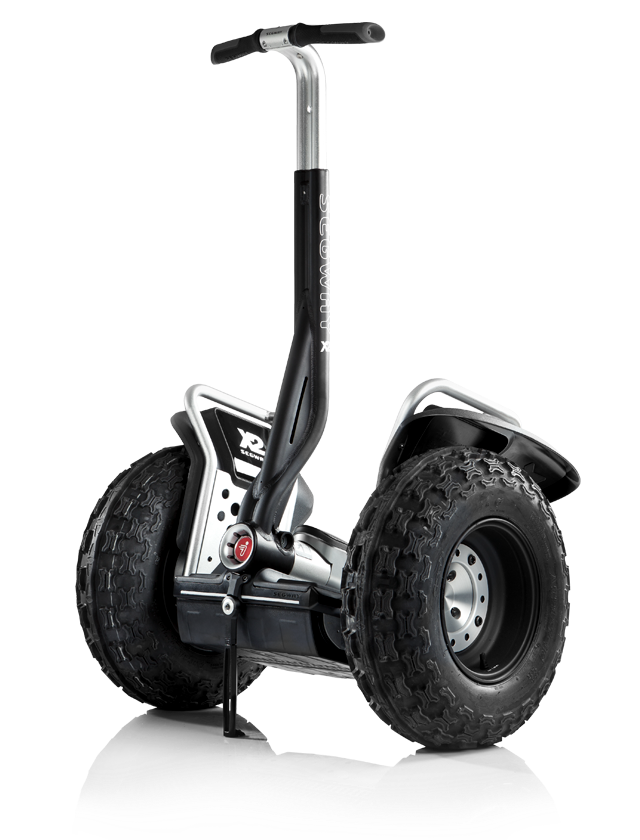
\includegraphics[width=\textwidth]{png/segway}

\textit{Segway\cite{segway}}
\end{center}
\end{minipage}\hfill
\begin{minipage}[c]{.22\linewidth}
\begin{center}
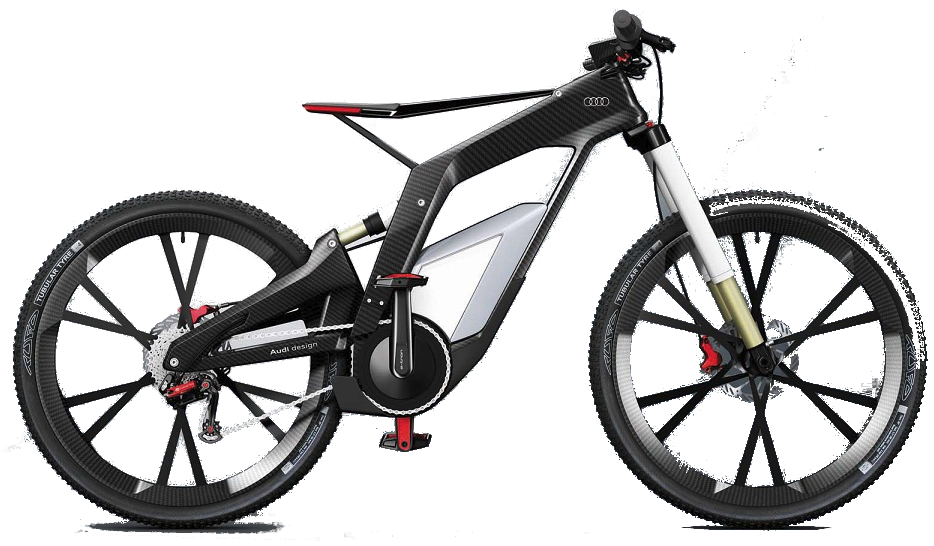
\includegraphics[width=\textwidth]{png/velo_audi}

\textit{Vélo électrique Audio \cite{audi}}
\end{center}
\end{minipage}

Il est donc important que les attentes du client soient spécifiées en détail afin que le produit industriel soit en phase avec les besoins de l'utilisateur. 


\end{exemple}



%\begin{defi}
%\textbf{Service attendu}
%
%\end{defi}
%
%
%\begin{exemple}
%\end{exemple}

\begin{defi}
\textbf{Exigence} \cite{roques}

Une exigence permet de spécifier une capacité ou une contrainte qui doit être satisfaite par un système. Elle peut spécifier une fonction que le système devra réaliser ou une condition de performance, de fiabilité, de sécurité, \textit{etc}.

Les exigences servent à établir un contrat entre le client et les réalisateurs du futur système.

\end{defi}

\begin{rem}
Une façon de structurer les exigences est de les trier ainsi :
\begin{itemize}
\item exigences fonctionnelles;
\item exigences légales;
\item exigences environnementales;
\item exigences techniques;
\item exigences pratiques;
\item exigences énergétiques;
\item exigences marketing;
\item \textit{etc.}
\end{itemize}
\end{rem}


%\begin{defi}
%\textbf{Spécifications fonctionnelles}
%
%\end{defi}
%
%\begin{exemple}
%\end{exemple}


\begin{defi}
\textbf{Cahier des charges fonctionnel} \cite{norme}

Document par lequel le demandeur exprime ses besoins (ou ceux qu'il a la charge d'exprimer) en terme de fonctions de service et de contraintes. Pour chacune d'elles sont définis des critères d'appréciation ainsi que leur niveaux, chacun d'entre eux étant assorti d'un certain degré de flexibilité.  

\textbf{Spécifications fonctionnelles}

Le cahier des charges peut donc interpréter comme une liste de spécifications fonctionnelles auxquelles le système doit répondre.

\end{defi}

\begin{exemple}
\textit{Satellite d'observation géophysique DEMETER}



\noindent\begin{minipage}[c]{.25\linewidth}
\begin{center}
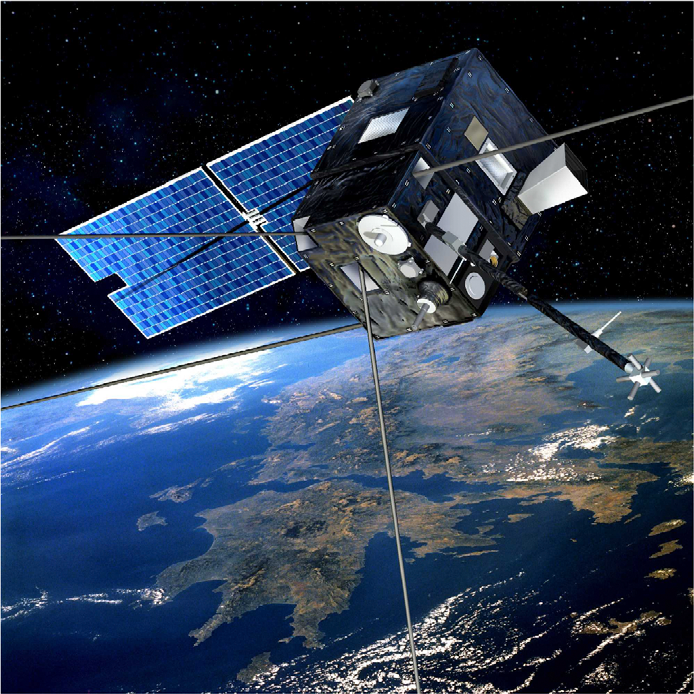
\includegraphics[width=.9\textwidth]{png/demeter}
\end{center}
\end{minipage}\hfill
\begin{minipage}[c]{.7\linewidth}
L’orbite choisie pour DEMETER impose que ses panneaux solaires ne captent la lumière du Soleil que
pendant une durée limitée à chaque révolution. Le courant n’est généré par les cellules des panneaux que
pendant ces périodes éclairées qui permettent alors de recharger le système de batteries. 
\end{minipage}

\begin{center}
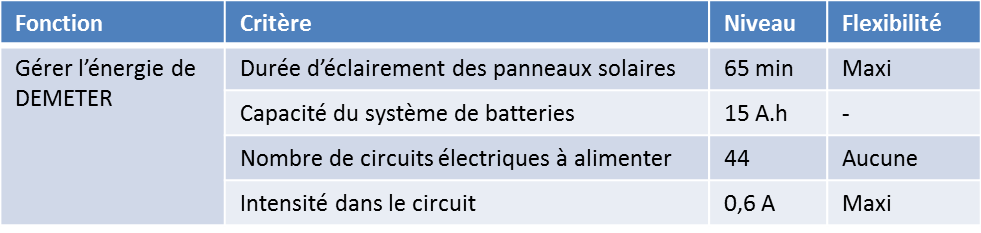
\includegraphics[width=.75\textwidth]{png/cdc_demeter}
\end{center}
\end{exemple}




\begin{defi}
\textbf{Solution technique}

La solution technique correspond au choix adopté par l'industriel pour répondre au besoin du client et aux exigences. 

\end{defi}

\begin{exemple}
Les Vibram fivefingers, le Magsurf, le Segway ou le vélo électrique Audi sont trois solutions techniques permettant de se rendre au Mourillon.
\end{exemple}


\section{Cycle de vie}
\subsection{Définitions}

On peut considérer le cycle de vie d'un produit comme l'enchaînement des étapes ci-dessous. 
\begin{center}
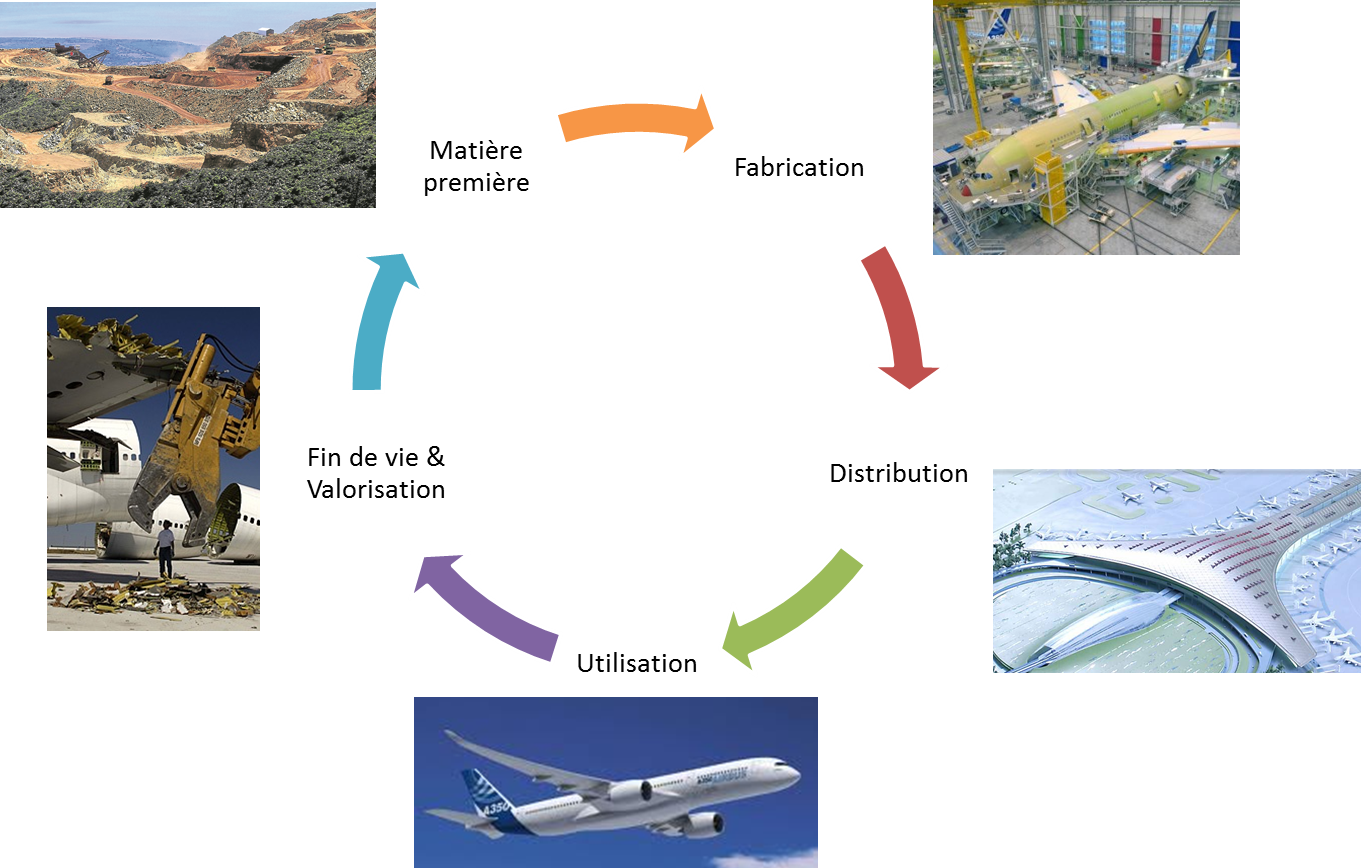
\includegraphics[width=.8\textwidth]{png/cycle_vie}
\end{center}


Chacune des étapes consomme des ressources et a un impact certain sur l'environnement. Les ressources naturelles n'étant pas inépuisables et l'impact de la pollution humaine impactant toujours plus les écosystèmes, il devient nécessaire de limiter l'impact des produits sur l'environnement. C'est ce qu'on appelle l'éco-conception. 

\noindent\begin{minipage}[c]{.47\linewidth}
\begin{center}
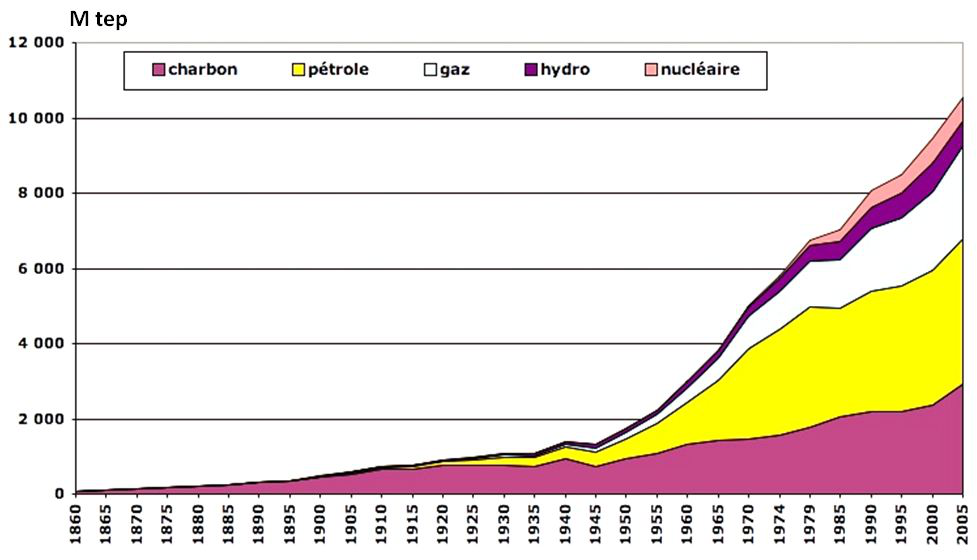
\includegraphics[height=5cm]{png/consommation_energie}

\textit{Consommation mondiale en millions de tonnes équivalent pétrole. Schilling \& Al}
\end{center}
\end{minipage}\hfill
\begin{minipage}[c]{.47\linewidth} 
\begin{center}
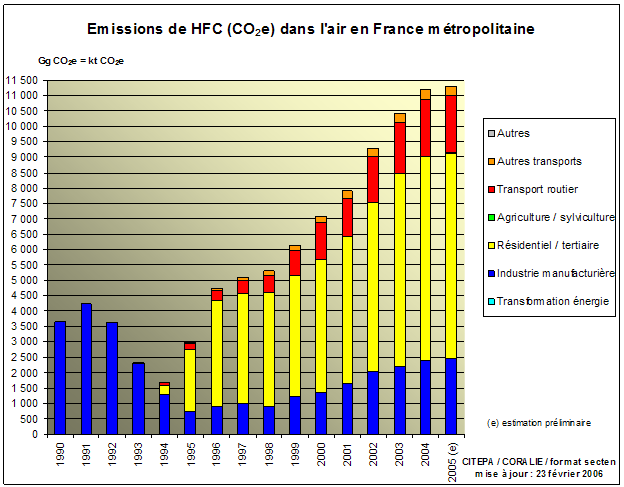
\includegraphics[height=6cm]{png/emission_CO2}

\textit{Emissions de CO2 en France métropolitaine}
\end{center}
\end{minipage}


\subsection{Impact environnemental}

Les impacts environnementaux sont classés en 3 familles d'impact :
\begin{itemize}
\item ressources naturelles non renouvelables; 
\item pollutions;
\item nuisances.
\end{itemize}

A chaque impact correspond alors une substance ou une unité de référence. 

\begin{center}
\begin{tabular}{|p{.2\textwidth}|p{.35\textwidth}|p{.35\textwidth}|}
\hline 
\textbf{Familles d’impacts} & \textbf{Impacts} & \textbf{Substance ou unité de référence} \\ \hline \hline 
\multirow{2}{.2\textwidth}{Ressources naturelles non renouvelables} & 
Consommation d’énergie non renouvelable & 
MégaJoule (\textit{MJ}) \\ \cline{2-3}
& Consommation de ressources naturelles non renouvelables  &
Antimoine ($Sb$) \\ \hline
Pollutions & 
Gaz à Effet de Serre (GES) ou Global Warming Potential (GWP) & 
Dioxyde de carbone ($CO_2$) \\ \cline{2-3}
&
Acidification liée aux pluies acides &
Dioxyde de soufre ($SO_2$) \\ \cline{2-3}
&
Eutrophisation : enrichissement excessif des milieux aquatiques en sels nutritifs &
Composé phosphaté ($PO_4^{3-}$) \\ \cline{2-3}
&
Dégradation de la couche d’ozone &
Fréon 11 (CFC-11) \\ \cline{2-3}
&
Toxicité d’une substance sur l’être humain ou sur les autres organismes (écotoxicité)&
1,4 Dichlorobenzène (1,4 DCB) \\ \hline
Nuisances & 
Acoustiques & 
Decibel (dB) \\
&& Seuil de danger à 90 dB (klaxon) \\ \cline{2-3}
& Visuelles & \\ \cline{2-3}
& Olfactives & \\
\hline
\end{tabular}
\end{center}

Afin de pouvoir comparer les différents impacts environnementaux, on peut par exemple déterminer le taux de $CO_2$ équivalent émis. 

\begin{center}
\begin{tabular}{|l|l|}
\hline
\textbf{Matériau} & \textbf{Émissions équivalentes de $CO_2$ en kg par tonne produite} \\ \hline \hline
Verre bouteille & 120 \\ \hline
Ciment & 250 \\ \hline
Acier & 300 à 850 selon le pourcentage de ferrailles \\ \hline
Verre plat & 400 \\ \hline
Papier-carton & 300 à 500 \\ \hline
Plastiques (polyéthylène, polystyrène, PCV, PET...)  & 500 à 1600 \\ \hline
Aluminium & 600 à 3000 selon le pourcentage de déchets d'aluminium \\ \hline
\end{tabular}
\end{center}


\subsection{Analyse du cycle de vie}
\begin{defi}
\textbf{Analyse du cycle de vie}

L'Analyse du Cycle de Vie réalise un bilan détaillé et quantitatif des entrées et des sorties mesurées aux frontières d'un produit. Cette analyse peut prendre en compte différents critères ou impact et les différentes étapes du cycle de vie mais afin de prendre en compte la notion de transfert d’impact, l’analyse multicritère / multi-étape est la plus pertinente.

Ainsi, pour chacune des étapes du cycle de vie d'un produit, il faut recenser les flux de matières et d'énergie. Les impacts environnementaux sont ensuite quantifiés sur l’ensemble du cycle de vie. 
\end{defi}

\begin{exemple}

\textit{Cafetière}
\begin{center}
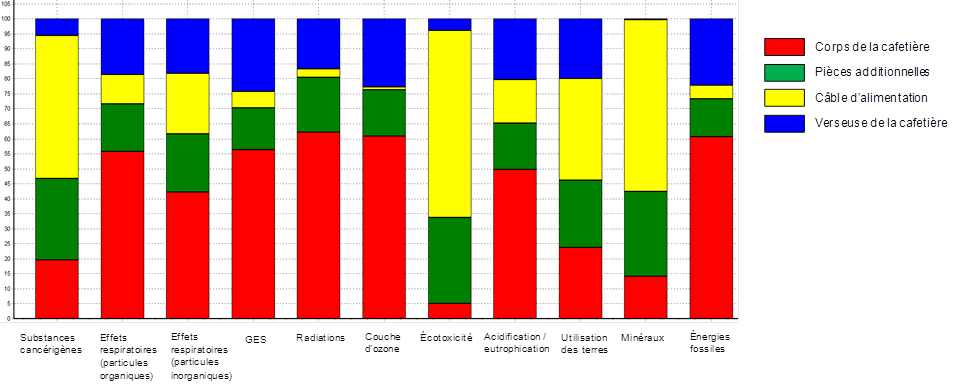
\includegraphics[width=.8\textwidth]{png/acv1}
\end{center}

Toutes les catégories d’impacts sont à 100\% car ils n’ont pas la même unité.
Afin de faciliter l’interprétation des résultats, il convient d’analyser l’importance des impacts en termes de contribution par rapport aux contributions globales. Par exemple, les émissions qui contribuent à l’acidification dans l’ACV sont-elles significatives par rapport aux émissions globales qui contribuent à l’acidification ?

C’est la phase de normalisation : les différentes familles d’impacts sont comparées avec les effets environnementaux causés par un européen moyen sur une année.

Les facteurs de normalisation représentent les émissions / consommations globales pendant un an sur une zone géographique donnée. Les résultats sont divisés par ce facteur, ce qui permet d’avoir une quantification de l’importance de l’émission par rapport aux émissions totales.

\begin{center}
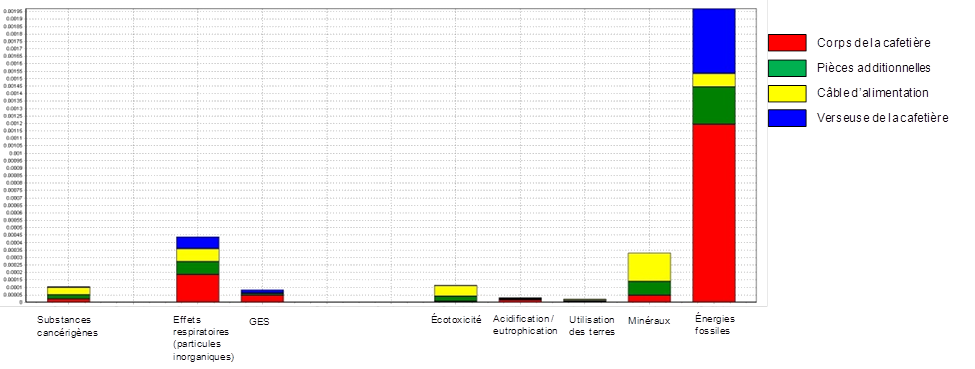
\includegraphics[width=.8\textwidth]{png/acv2}
\end{center}

L’étape suivante est la pondération qui consiste à donner plus de poids aux impacts qui sont jugés plus « graves » : l’effet de serre est-il plus néfaste que l’épuisement des ressources ? Elle est de ce fait controversée car il s’agit de pondérer puis d’additionner des impacts de natures différentes, nécessitant des partis-pris importants parfois considérés comme arbitraires.

\begin{center}
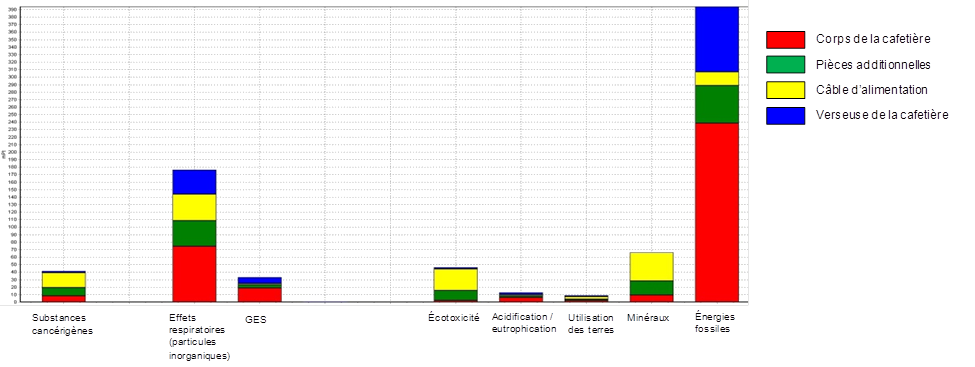
\includegraphics[width=.8\textwidth]{png/acv3}
\end{center}

\end{exemple}

\section{Ingénierie Système}

\subsection{Industrialisation des systèmes}
\subsubsection{Cycle d'industrialisation}
Le cycle d'industrialisation d'un système complexe peut être schématisé selon la figure suivante.

\begin{center}
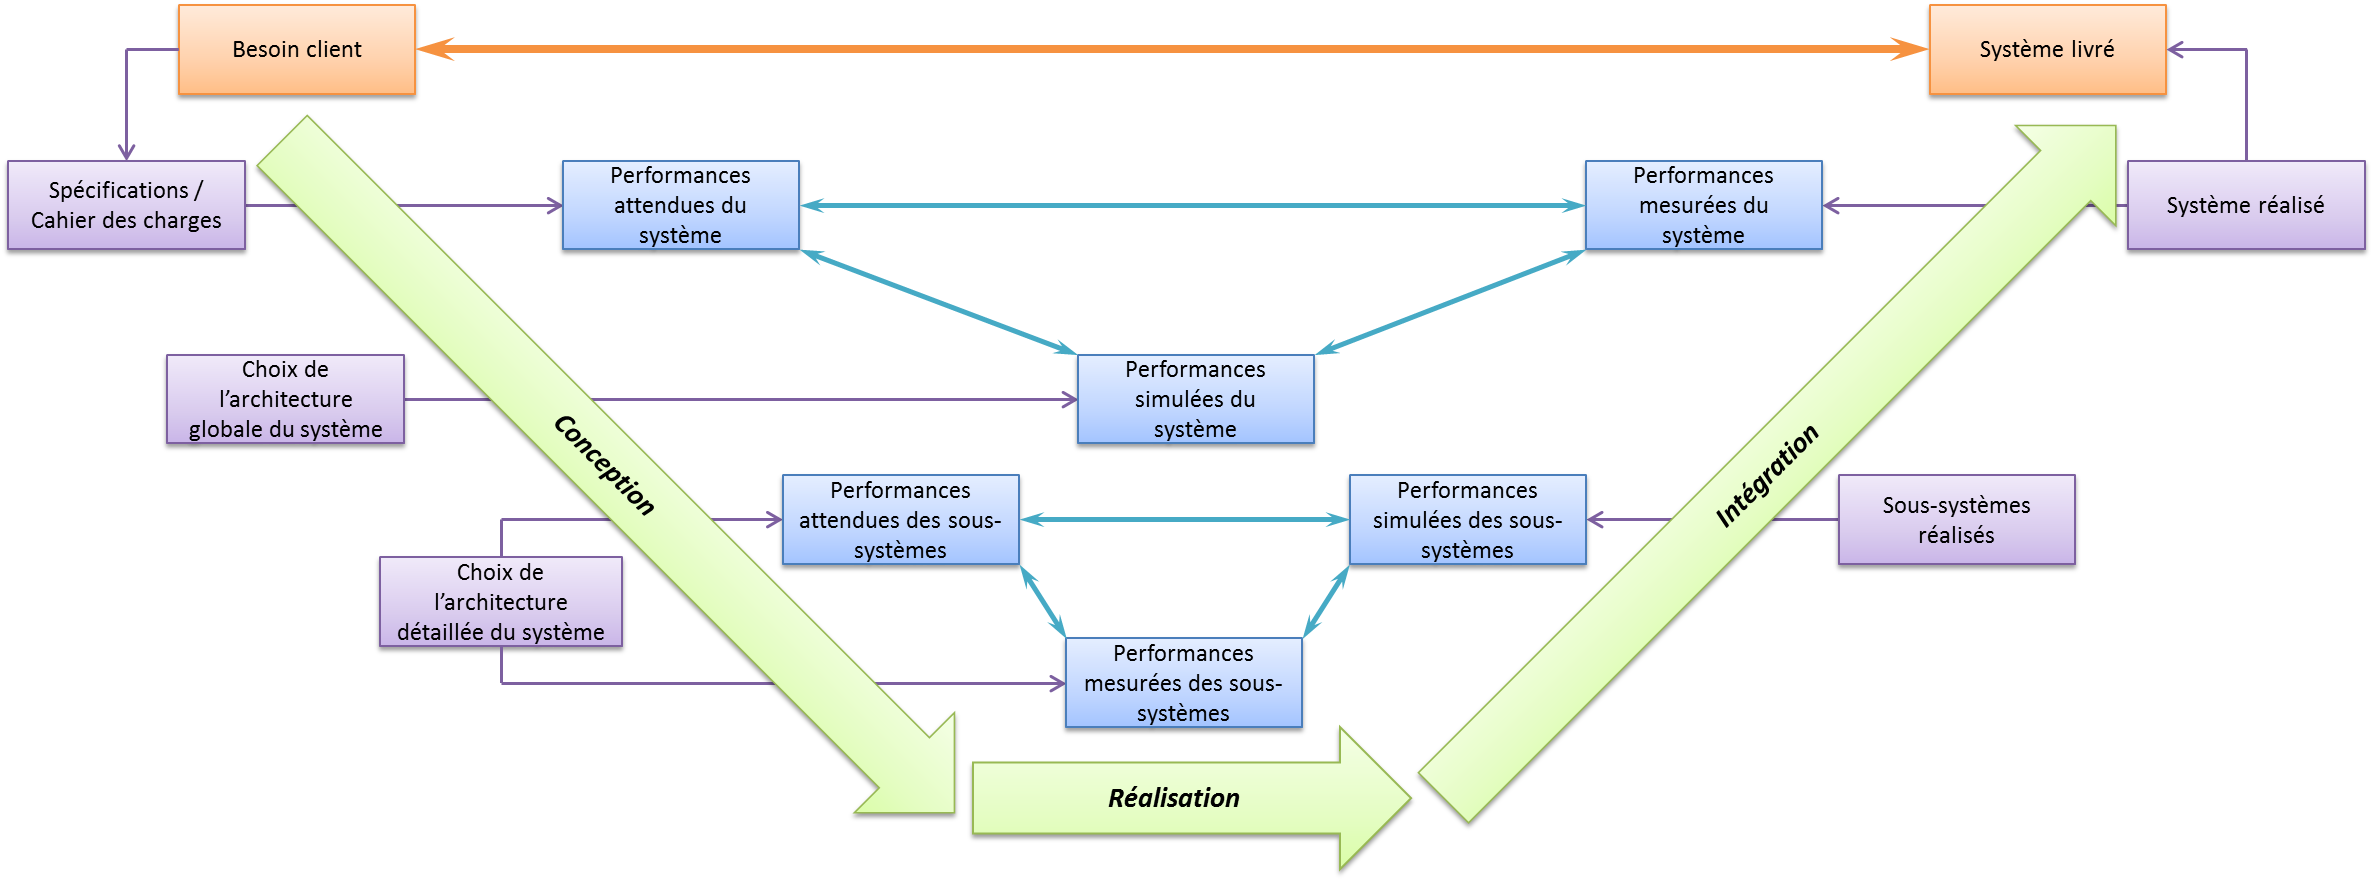
\includegraphics[width=\textwidth]{png/cycle}
\end{center}

\begin{prob}
Les principaux problèmes de l'ingénierie système pourraient être résumés ainsi :

\textbf{Comment faire en sorte que le système livré par l'industriel soit en adéquation avec les besoins du client ?}

\textbf{Comment faire en sorte, à chaque étape de l'industrialisation que les écarts entre le produit en cours d'industrialisation et le produit souhaité par le client soient minimums ?}
\end{prob}

En effet, la vie des entreprises dépend de la vente des produits fabriqués. Il est donc indispensable de faire en sorte que tout soit fait pour définir au mieux le besoin du client afin de le satisfaire. 


\subsubsection{Industrialisation d'un produit}
\begin{defi}
\textbf{Conception}

La conception désigne l'ensemble des travaux et des études mise en \oe{}uvres en vu de la réalisation d'un produit conforme aux exigences énoncées.


\textbf{Conception assistée par ordinateur (CAO)}

La CAO permet de réaliser virtuellement les produits à fabriquer. Il peut s'agir de conception mécanique (conception de pièces unitaires puis d'assemblages), de conception électronique (conception de circuits imprimés), de conception architecturale \textit{etc}.

\end{defi}

\begin{exemple}
\textit{CAO -- Solidworks -- Moteur de modélisme}


\begin{minipage}[c]{.45\linewidth}
\begin{center}
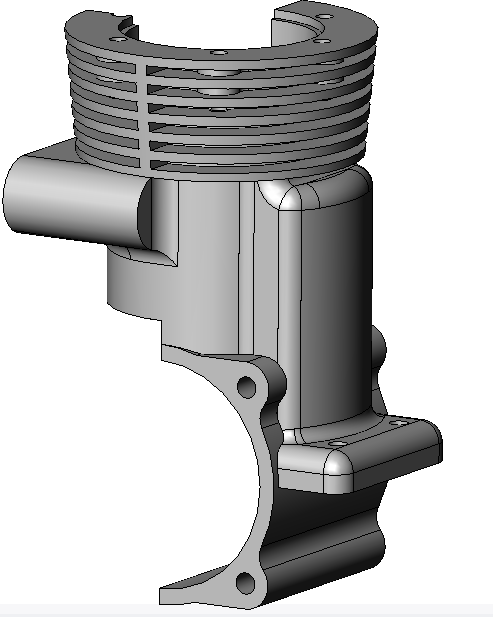
\includegraphics[width=.45\textwidth]{png/carter}

\textit{Carter de moteur de modélisme (vue coupée)}
\end{center} 
\end{minipage} \hfill
\begin{minipage}[c]{.45\linewidth}
\begin{center}
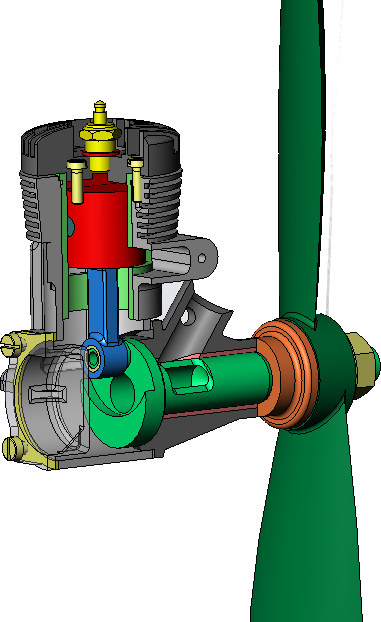
\includegraphics[width=.45\textwidth]{png/micromoteur}

\textit{Micromoteur de modélisme (vue coupée)}
\end{center} 
\end{minipage} 




\end{exemple}

\begin{rem}
Dans l'industrie, la conception totale d'un produit est relativement rare. Les nouveaux produits fabriqués sont souvent des évolutions de produits existants. 
\end{rem}

\begin{defi}
\textbf{Simulation}

Afin de valider le choix des composants d'un système ainsi que leur bon dimensionnement, il est nécessaire de faire des essais. Devant la complexité et le coût de réalisation des essais, les ingénieurs ou les chercheurs utilisent des outils permettant de modéliser grâce à des logiciels le comportement réel des systèmes. 

La simulation permet donc de vérifier le comportement d'un système sans faire d'expérimentation.
\end{defi}

\begin{prob}
Le bon résultat d'une simulation dépend étroitement de la qualité des modèles. Or il est parfois très difficile de modéliser les systèmes complexes. Il faut systématiquement garder un esprit critique vis-à-vis des logiciels de simulation.
\end{prob}

\newpage

\begin{exemple}
\noindent\begin{minipage}[c]{.45\linewidth}
\begin{center}
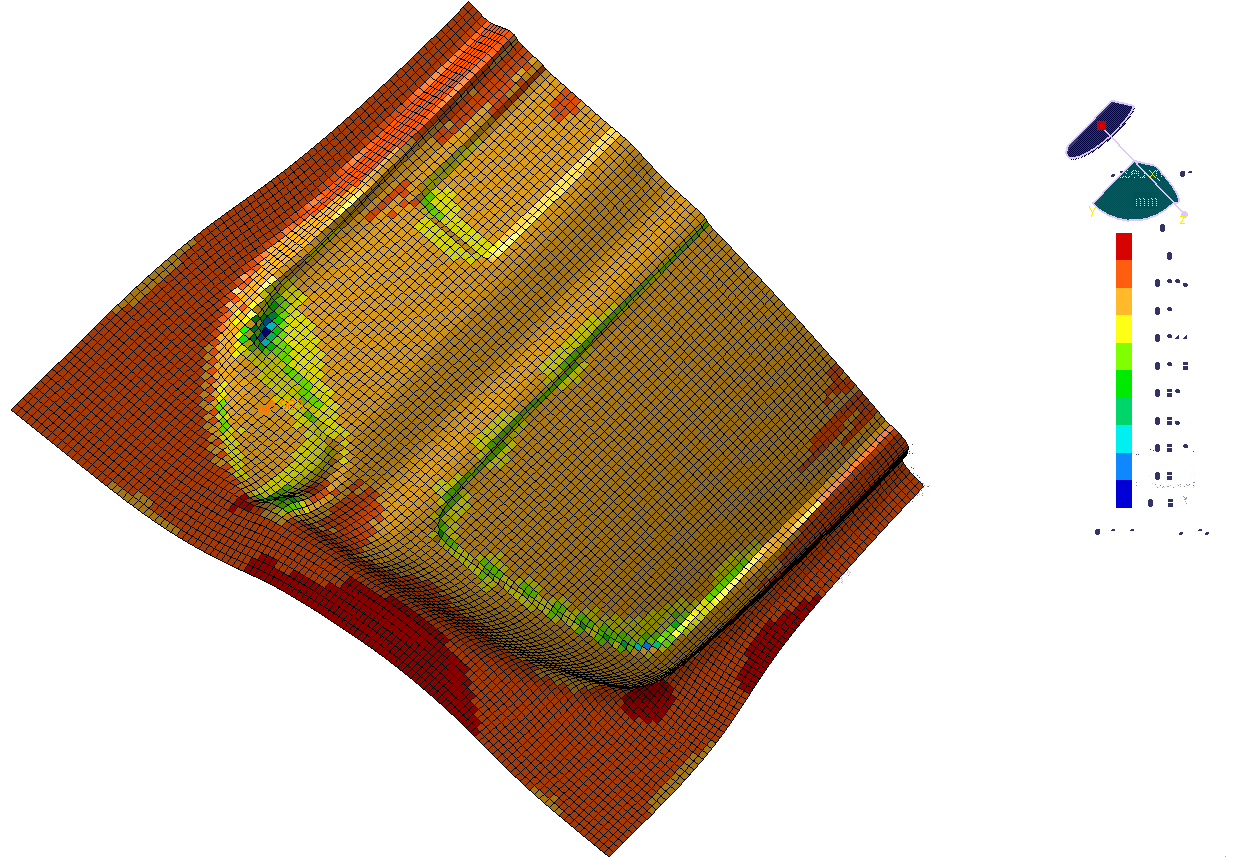
\includegraphics[width=\textwidth]{png/simu_emboutissage}

\textit{Simulation d'une opération d'emboutissage}\cite{embouti}
\end{center}
\end{minipage} \hfill
\begin{minipage}[c]{.45\linewidth}
\begin{center}
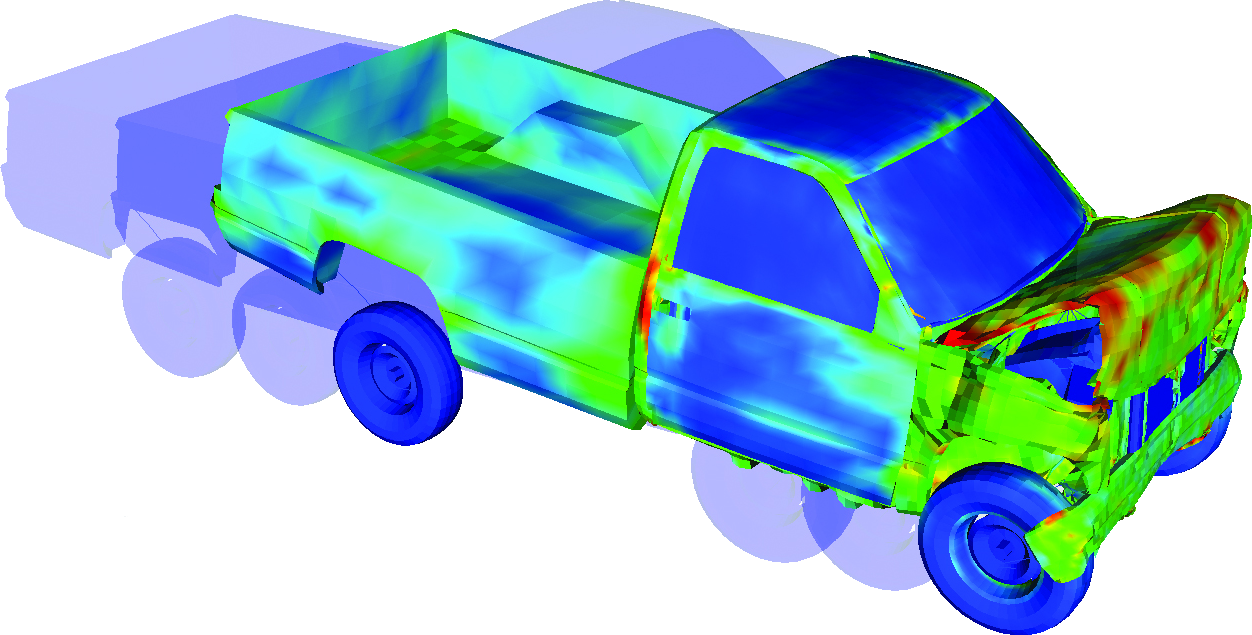
\includegraphics[width=\textwidth]{png/crash}

\textit{Simulation d'un crash par éléments finis}\cite{ef}
\end{center}
\end{minipage}


\noindent\begin{minipage}[c]{.35\linewidth}
\begin{center}
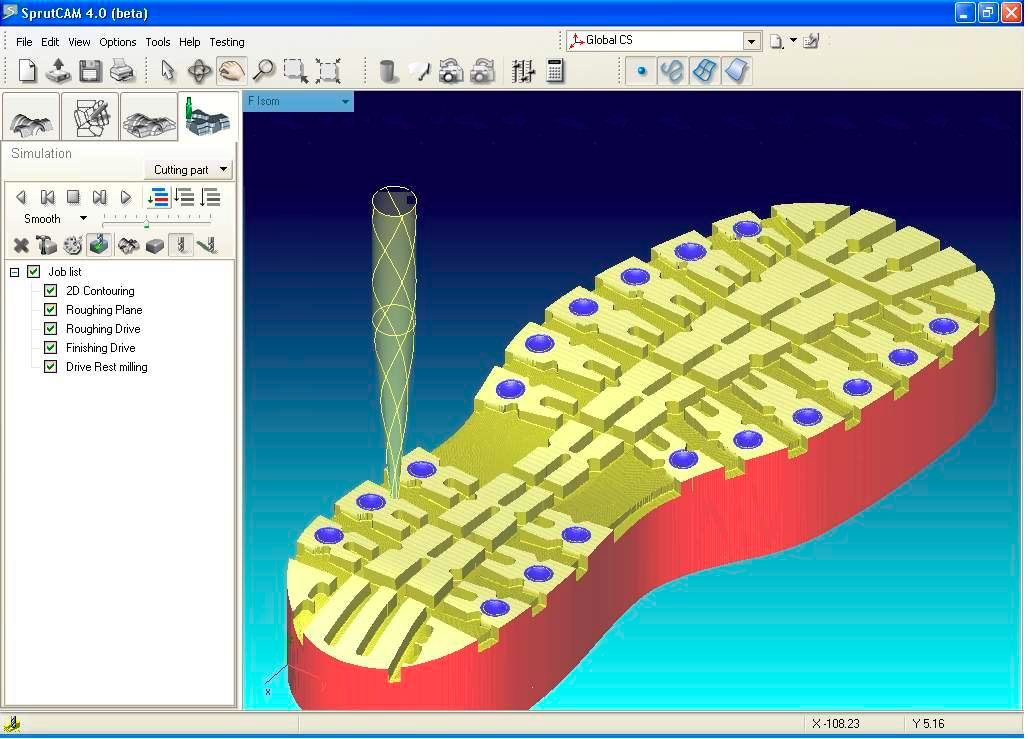
\includegraphics[width=\textwidth]{png/FAO}

\textit{Simulation d'une opération de Fabrication Assistée par Ordinateur}\cite{fao}
\end{center}
\end{minipage} \hfill
\begin{minipage}[c]{.55\linewidth}
\begin{center}
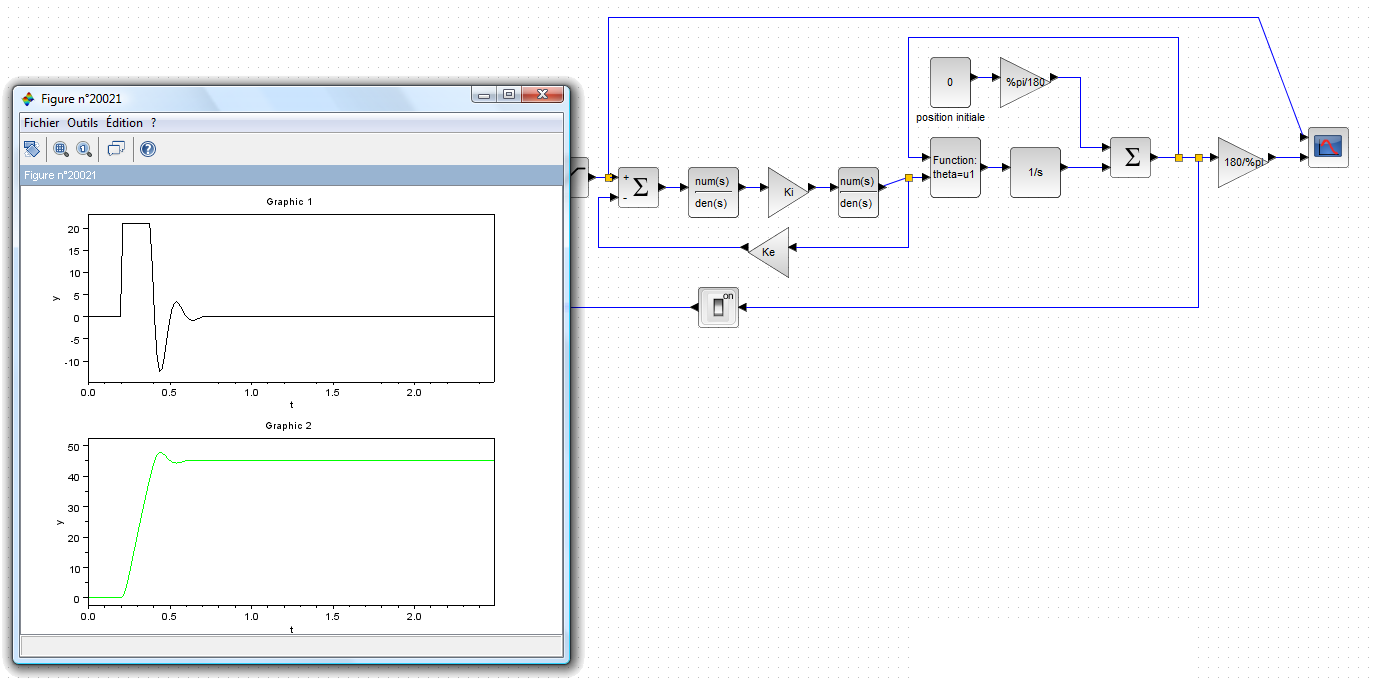
\includegraphics[width=\textwidth]{png/scilab}

\textit{Simulation multiphysique avec Scilab-XCOS}\cite{scilab}
\end{center}
\end{minipage} 
\end{exemple}

\begin{defi}
\textbf{Réalisation}

La réalisation comprend toutes les étapes permettant l'extraction de la matière première jusqu'à l'assemblage des parties mécaniques et électroniques. 
\end{defi}

\begin{exemple}

\begin{minipage}[c]{.22\linewidth}
\begin{center}
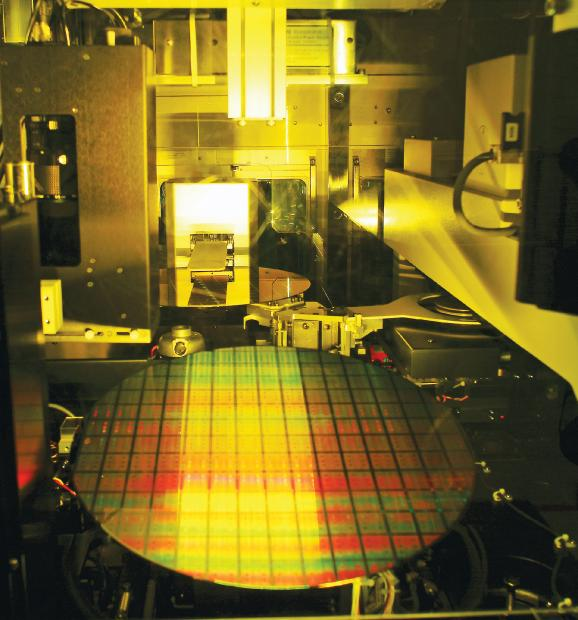
\includegraphics[width=.95\textwidth]{png/wafer2}

\textit{Chaîne de fabrication d'un Wafer de Silicium}\cite{wafer}
\end{center}
\end{minipage}
\hfill
\begin{minipage}[c]{.22\linewidth}
\begin{center}
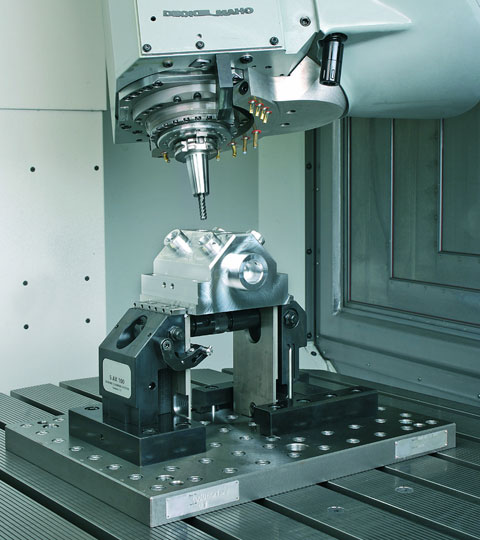
\includegraphics[width=.95\textwidth]{png/usinage}

\textit{Centre d'usinage 5 axes}\cite{u5x}
\end{center}
\end{minipage}
\hfill
\begin{minipage}[c]{.22\linewidth}
\begin{center}
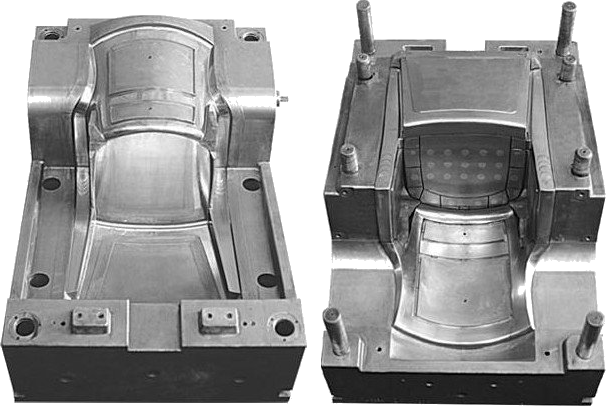
\includegraphics[width=.95\textwidth]{png/injection}

\textit{Moule d'injection plastique d'une chaise en ABS}\cite{injection}
\end{center}
\end{minipage}
\hfill
\begin{minipage}[c]{.22\linewidth}
\begin{center}
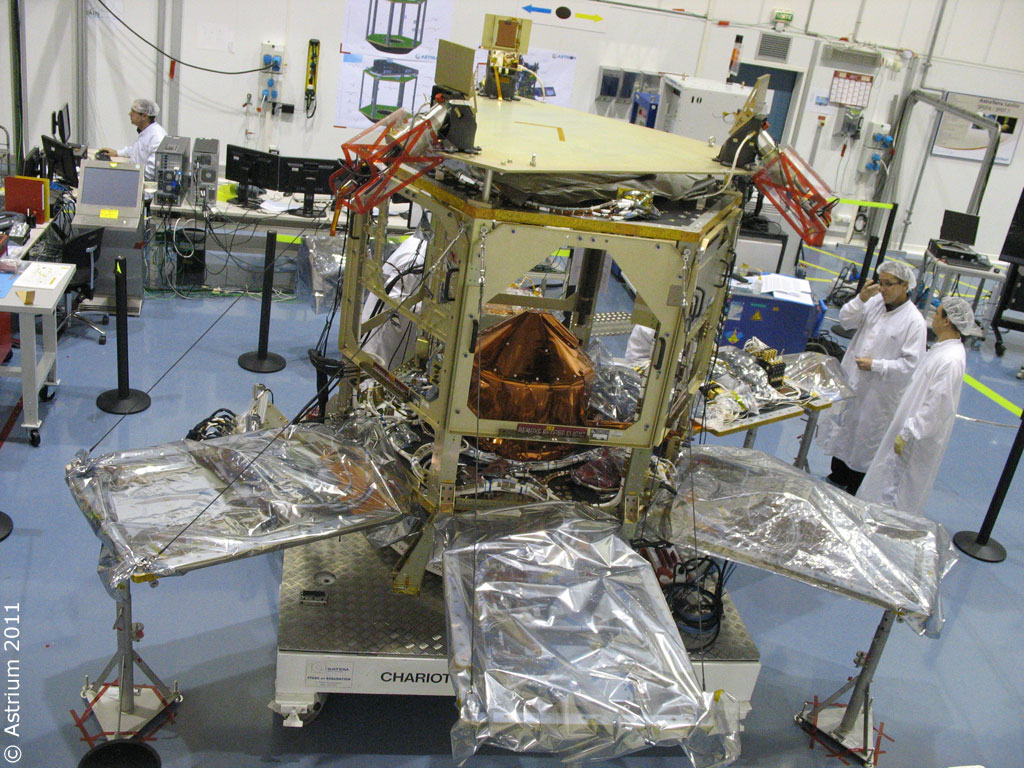
\includegraphics[width=.95\textwidth]{png/satellite}

\textit{Assemblage d'un satellite}\cite{satellite}
\end{center}
\end{minipage}

\end{exemple}

\begin{rem}
\textbf{Le triptyque Produit -- Procédé -- Matériau -- PPM}

\noindent\begin{minipage}[c]{.7\linewidth}
Comme tout le cycle d'industrialisation d'un produit, sa réalisation n'est pas un processus linéaire, mais est un fruit de compromis. On abordera le triptyque que PPM qui met en évidence que les choix des formes d'un produit, de matériaux et de procédés résultent de discussion nombreuses entre les différents bureau d'étude d'une entreprise. 
\end{minipage}\hfill
\begin{minipage}[c]{.25\linewidth}
\begin{center}
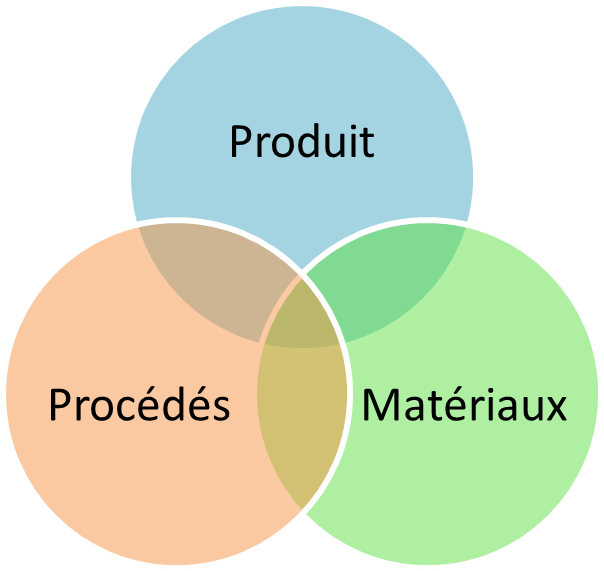
\includegraphics[width=.95\textwidth]{png/ppm}
\end{center}
\end{minipage}
\end{rem}

\begin{defi}
\textbf{Intégration}

L'intégration comprend les étapes de développement logiciel à savoir la création de l'architecture logicielle, la programmation, le débuggage, la mise en service du système et sa maintenance.
\end{defi}


\subsubsection{Performances d'un système}


L'ensemble du processus industriel va faire naître des écarts : 
\begin{itemize}
\item écarts entre les performances du produit imaginées par l'industriel et les performances du produit désiré par le client;
\item écarts entre les performances du produit conçu par le bureau d'étude et les performances du produit réalisé par l'atelier de fabrication;
\item écarts entre les simulations issues du bureau d'étude et les performances réelles du système;
\item entre les performances du produit commercialisé et les attentes du client.
\end{itemize}

Le but des Sciences Industrielles de l'Ingénieur (et des industriels) et de quantifier et maîtriser l'ensemble de ces écarts pour atteindre la satisfaction client la plus grande possible. 


\begin{center}
\begin{minipage}[c]{.47\linewidth}
\begin{center}
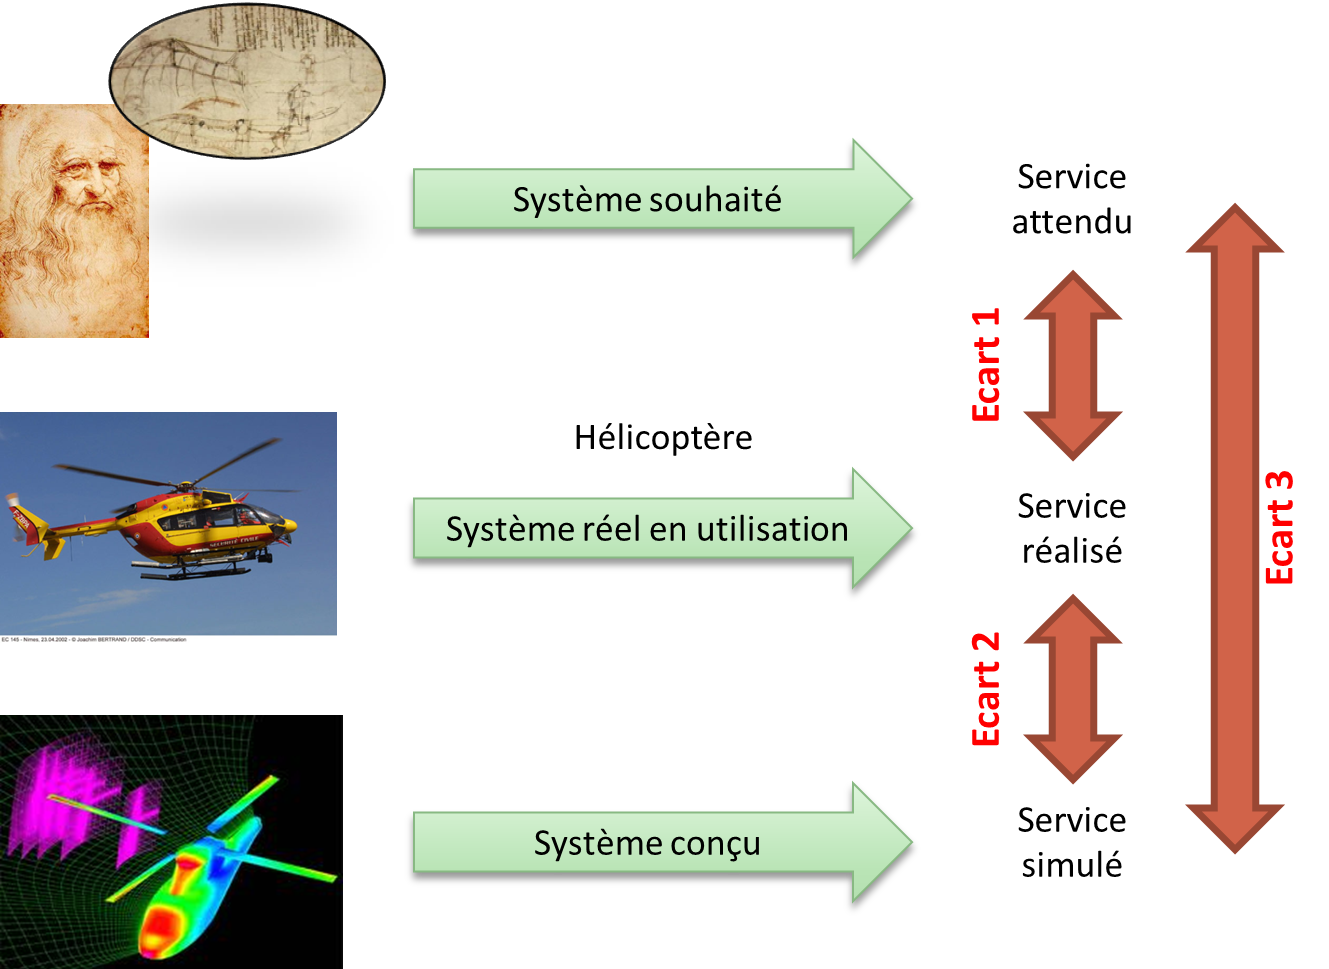
\includegraphics[width=\textwidth]{png/ecarts1}
\end{center}
\end{minipage}\hfill
\begin{minipage}[c]{.47\linewidth}
\begin{center}
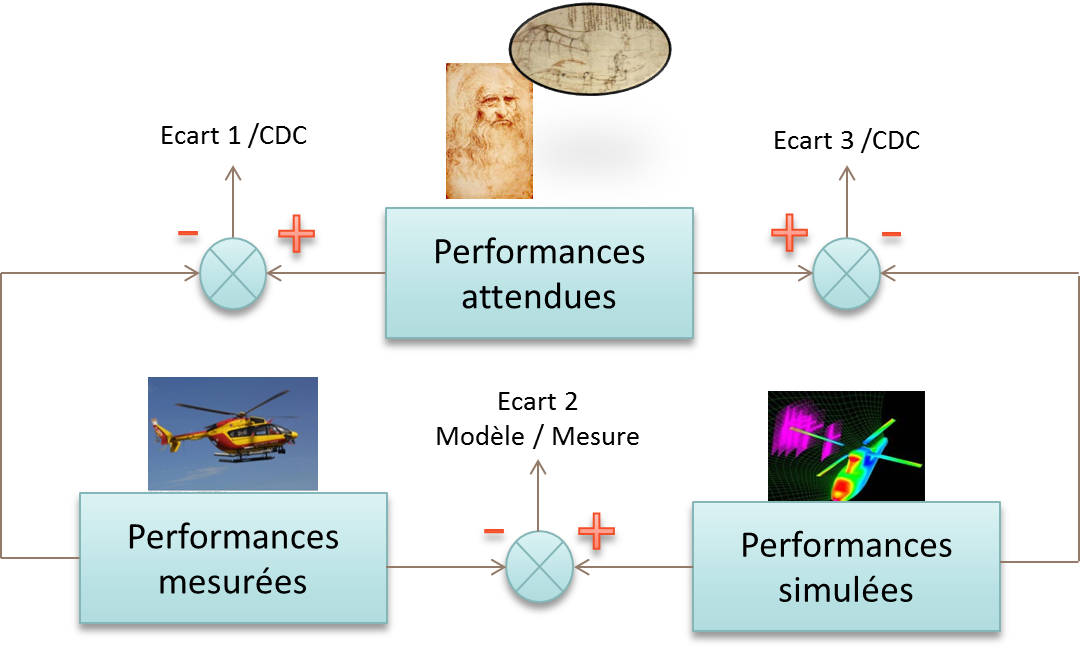
\includegraphics[width=\textwidth]{png/ecarts2}
\end{center}
\end{minipage}

\textit{Modélisation des écarts}
\end{center}

\subsection{Nécessité de l'Ingénierie Systèmes}

L'ensemble de ce qui a été énoncé précédemment touche du doigt les difficultés qui peuvent être liées à la réalisation d'un système. Aussi, il est nécessaire pour les entreprises de disposer de méthodes robustes pour faire en sorte que tous les acteurs participants à la réalisation d'un produit puissent \textbf{communiquer}. Les acteurs peuvent être les services marketing, le bureau d'étude, le bureau des méthodes, l'atelier de fabrication, les services commerciaux, financiers, innovations, clients, les diffuseurs, les réseaux de distribution...

\begin{defi}
\textbf{Ingénierie Système} \cite{roques}

Approche
interdisciplinaire rassemblant tous les efforts techniques pour faire évoluer et vérifier un
ensemble intégré de systèmes, de gens, de produits et de solutions de processus de
manière équilibrée au fil du cycle de vie pour satisfaire aux besoins client.

\end{defi}



\subsection{La modélisation SysML}


\begin{defi}
\textbf{Langage SysML} \cite{sii}

Le langage SysML a pour objectif de formaliser, de manière graphique et indépendante de
l’outil logiciel, les spécifications disparates associées à un système technique complexe.

Il permet, entre autres, de spécifier, concevoir, définir et analyser la structure d’un système,
identifier les performances, les limites, l’environnement et les relations avec l’extérieur. Il a
donc avant tout un objectif de documentation de la modélisation adoptée et n’est donc pas
une méthode d’étude, de réflexion ou de conception d’un produit industriel

\end{defi}


Le modèle SysML doit être un outil de communication utilisé dans toutes les phases de vie du produit afin que les différents acteurs puissent communiquer et mesurer les écarts entre le produit en cours de réalisation et les différentes exigences. 

Il peut être utilisé en phase de conception innovante, mais aussi en phase de reconception d'un produit déjà existant. Il facilitera ainsi les évolutions futures. 




Historiquement, le langage SysML dérive de l'UML (\textit{Unified Modeling Language}). L'UML est un langage de modélisation graphique utilisé lors du développements logiciels (en particulier lorsque les logiciels sont programmés en langage orienté Objet -- \textit{Python, JAVA, C++}). Pour cela 13 diagrammes différents sont utilisés répartis en 6 diagrammes structurels et 7 diagrammes comportementaux. 

Les besoins de l'ingénierie système et de l'ingénierie logicielle n'étant pas complètement identiques, le SysML reprend des diagrammes issus directement de l'UML et intègre de nouveaux diagrammes propres à la modélisation des systèmes (diagramme des exigences et diagramme paramétrique. 



\begin{center}
\noindent\rule[0.5ex]{.45\textwidth}{0.1mm} \hfill \cite{roques}\hfill 
\rule[0.5ex]{.45\textwidth}{0.1mm}
\end{center}


SysML s’articule autour de neuf types de diagrammes, chacun d’eux étant dédié à la
représentation des concepts particuliers d’un système. Ces types de diagrammes sont
répartis par l’OMG en trois grands groupes :
\begin{itemize}
\item quatre diagrammes comportementaux :
\begin{enumerate}
\item diagramme d’activité (montre l’enchainement des actions et décisions au sein d’une
activité complexe);
\item diagramme de séquence (montre la séquence verticale des messages passés entre
blocs au sein d’une interaction);
\item diagramme d’états (montre les différents états et transitions possibles des blocs
dynamiques);
\item diagramme de cas d’utilisation (montre les interactions fonctionnelles entre les
acteurs et le système à l’étude);
\end{enumerate}
\item un diagramme transverse : le diagramme d’exigences (montre les exigences du système
et leurs relations);
\item quatre diagrammes structurels :
\begin{enumerate}
\item diagramme de définition de blocs (montre les briques de base statiques : blocs,
compositions, associations, attributs, opérations, généralisations, etc.) ;
\item diagramme de bloc interne (montre l’organisation interne d’un élément statique
complexe) ;
\item diagramme paramétrique (représente les contraintes du système, les équations qui le
régissent) ;
\item diagramme de packages (montre l’organisation logique du modèle et les relations
entre packages).
\end{enumerate}
\end{itemize}

\noindent\rule[0.5ex]{\textwidth}{0.1mm}

\section{La modélisation SysML \cite{sii}}
Les différents diagrammes SysML seront vus en détail dans un autre document. Le but de cette partie est de présenter succinctement chacun des diagrammes.

\textbf{On s'intéresse ici à la modélisation SysML d'un drone multi-rotors utilisé pour la prise de vue aérienne lors de la réalisation de films ou de reportages.}
\begin{center}
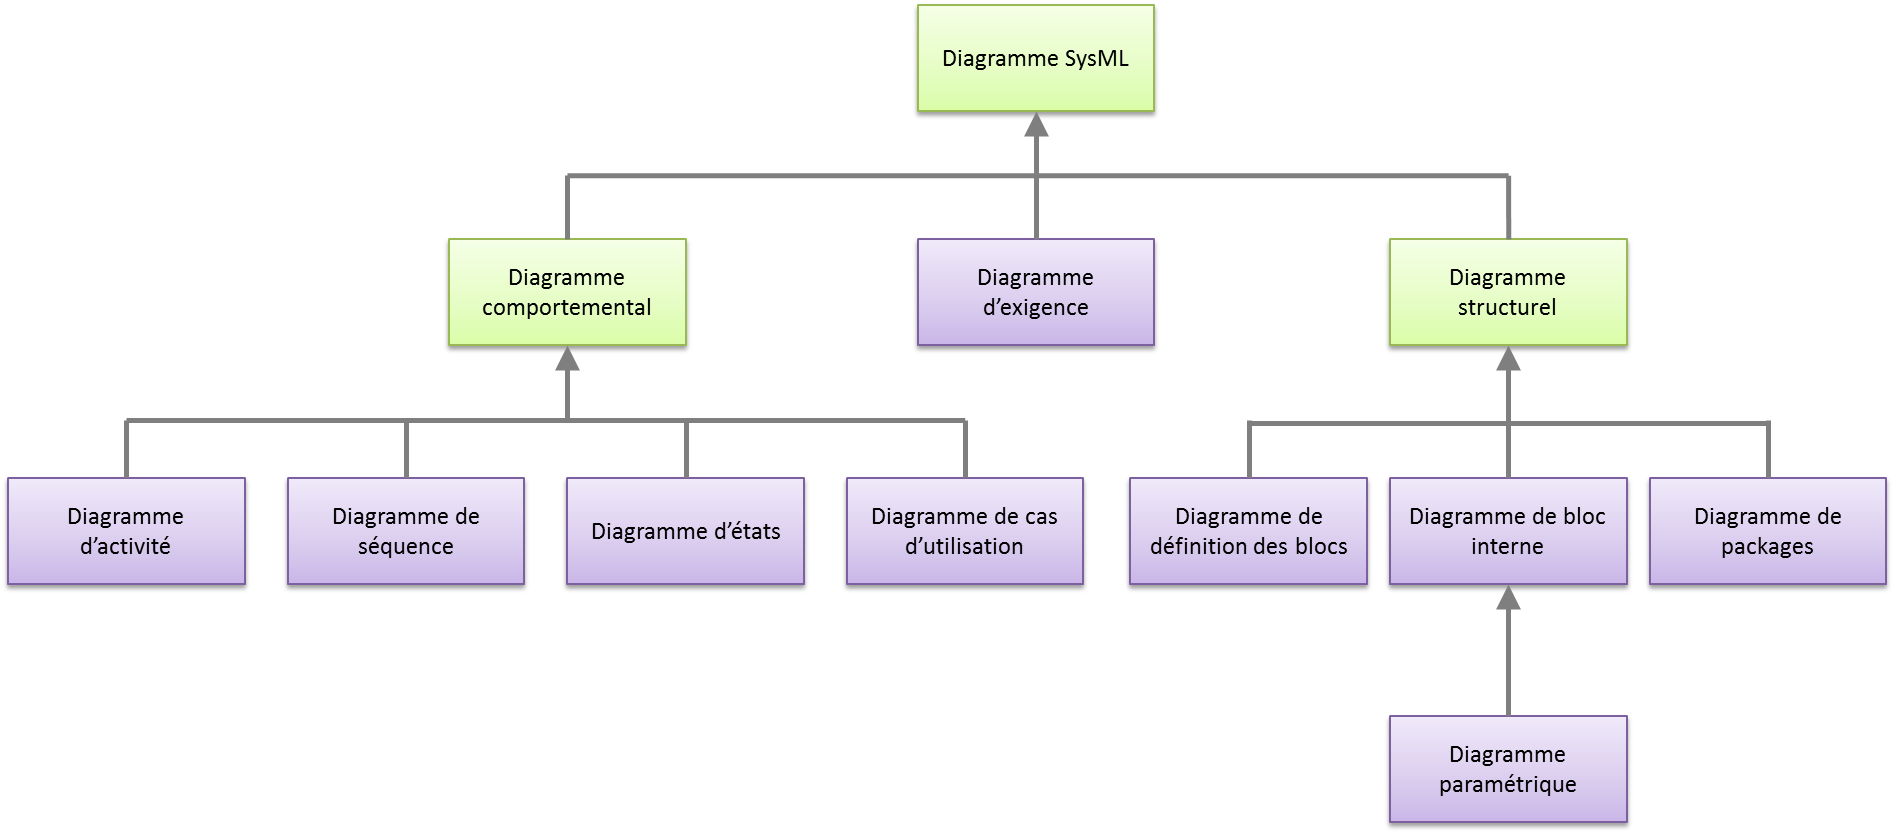
\includegraphics[width=\textwidth]{png/diagrammes_sysml}
\end{center}

\subsection{Diagramme des exigences}
\begin{defi}
\textbf{Diagramme des exigences -- \textit{Requirement Diagram -- req}}

L’objectif de ce diagramme est de modéliser les exigences devant être vérifiées par le
système en liant les solutions mises en \oe{}uvre sur le système avec les besoins définis dans le
cahier des charges. Ce diagramme traduit, par des fonctionnalités ou des contraintes, ce qui
doit être satisfait par le système.

De nombreux domaines peuvent être couverts, les plus classiques étant les exigences
environnementales, économiques, fonctionnelles ou techniques.
\end{defi}

\begin{exemple}
\begin{center}
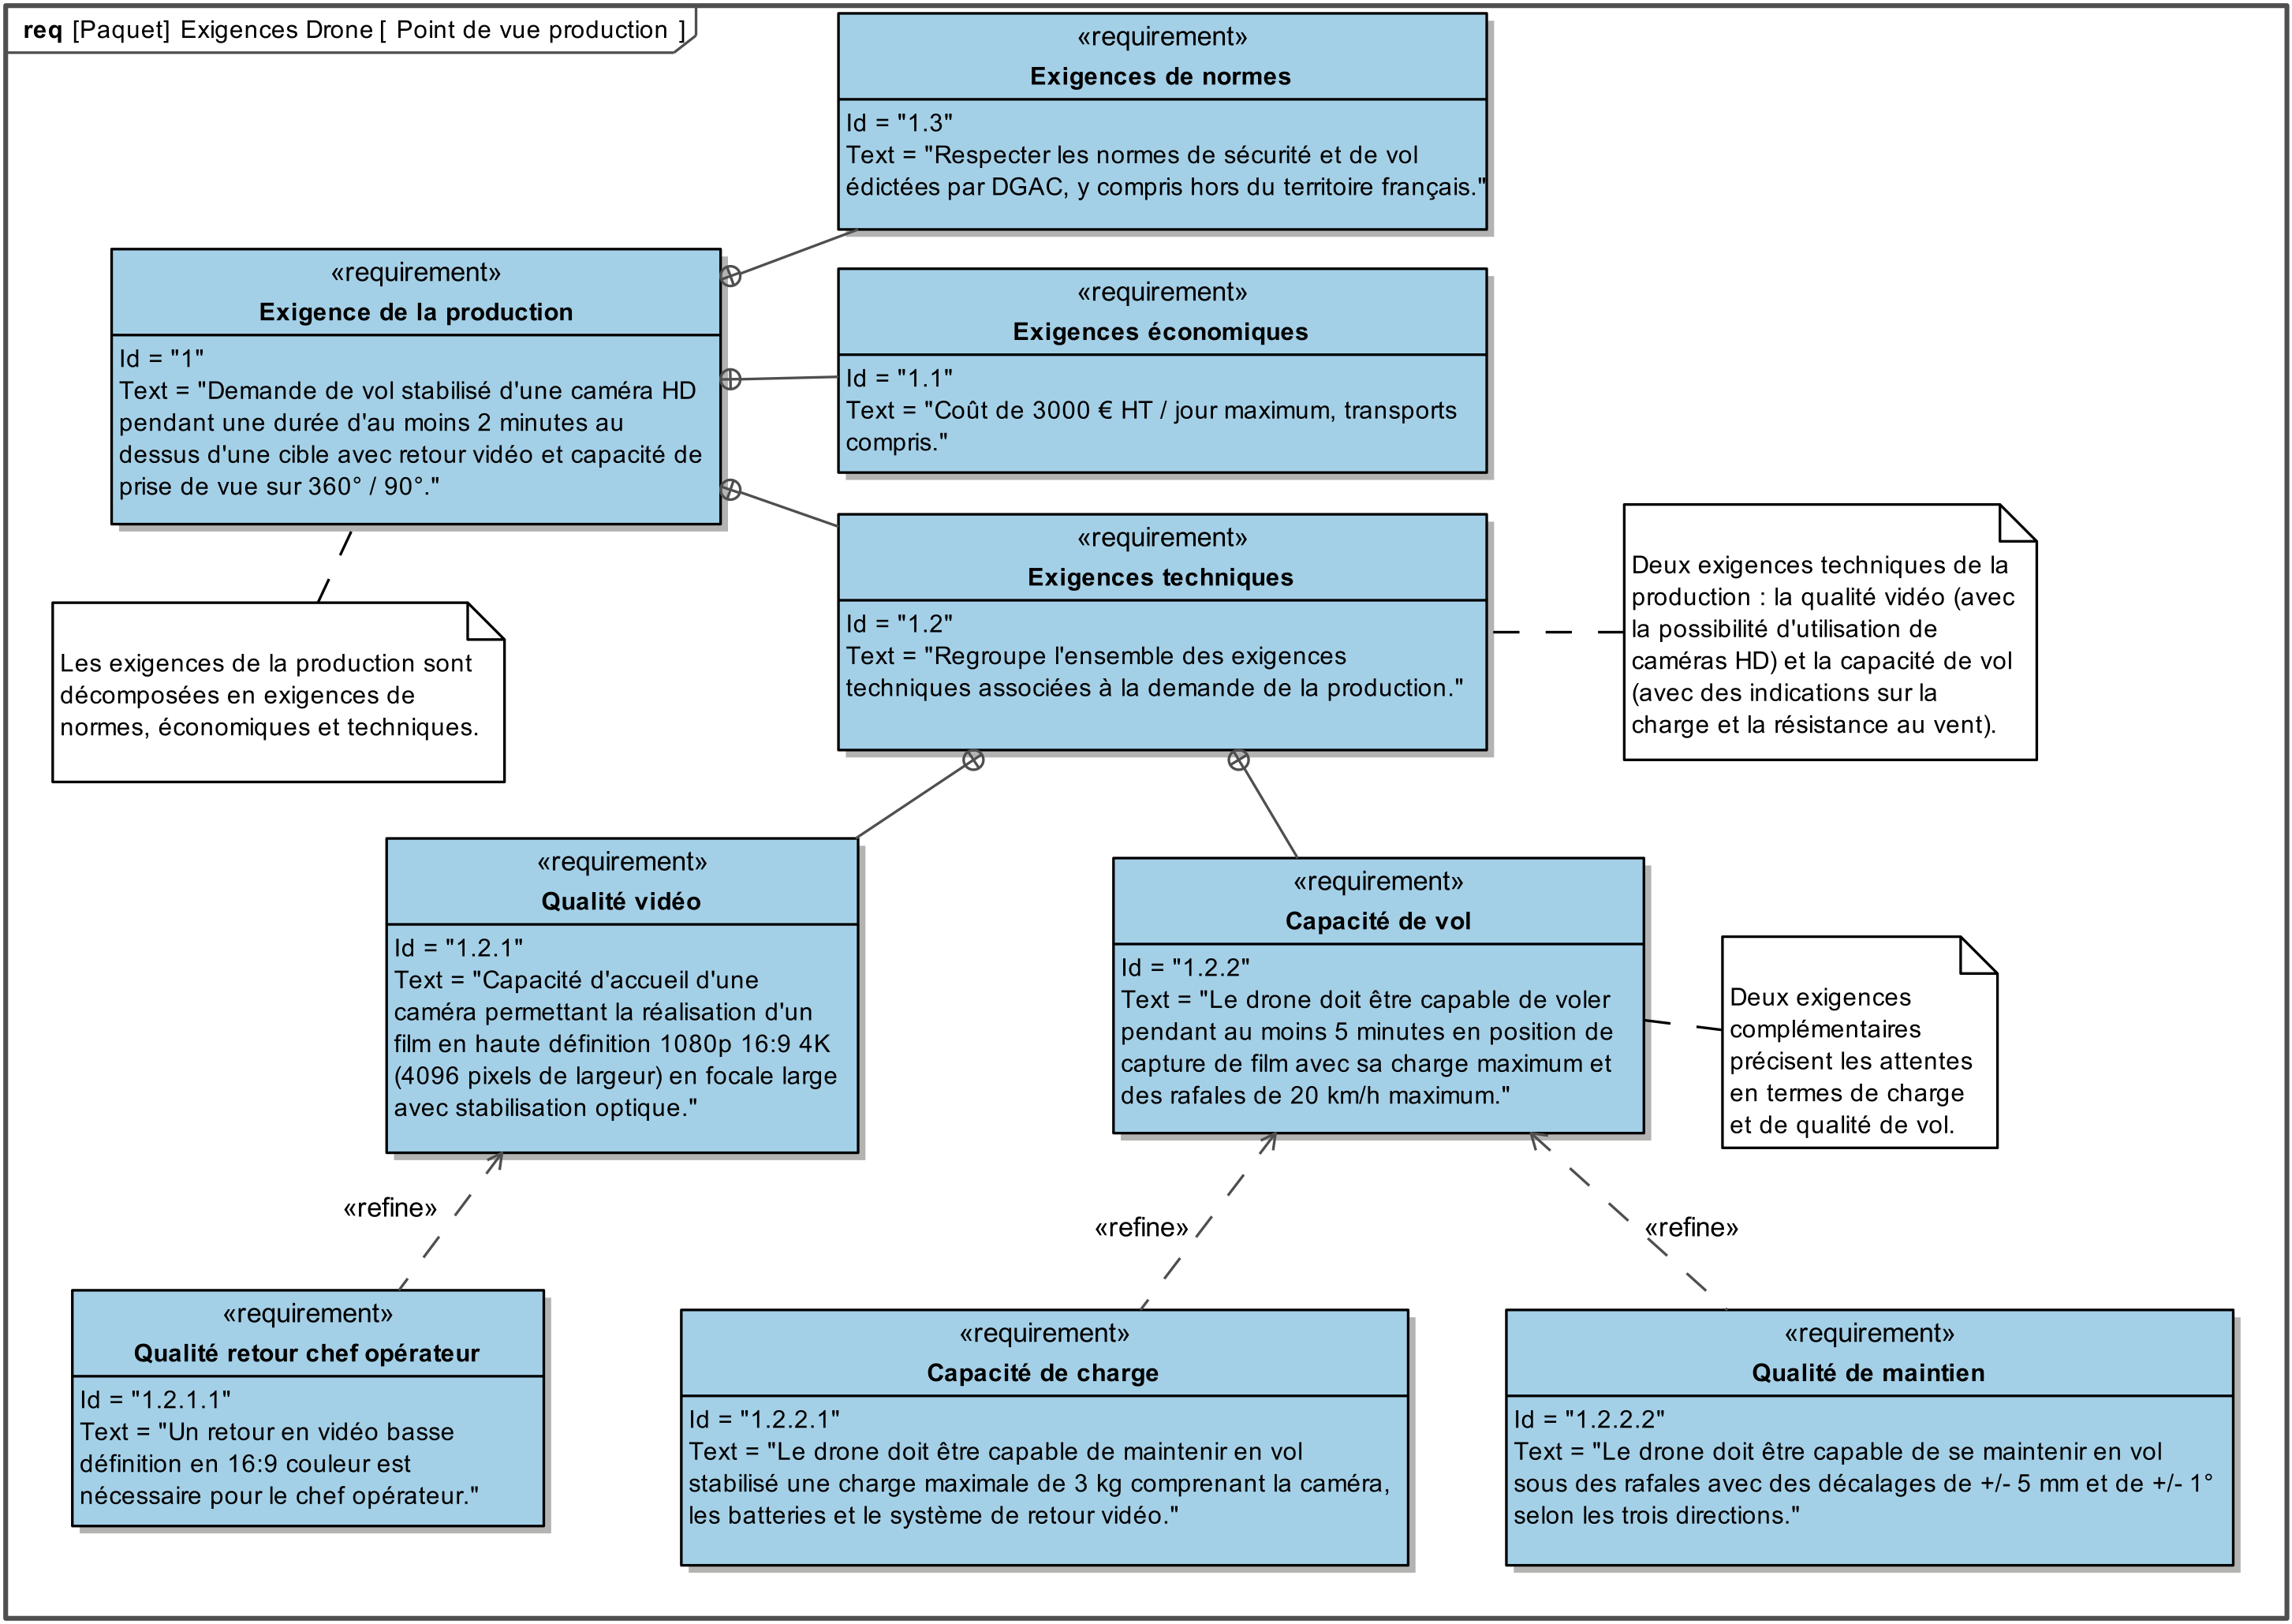
\includegraphics[width=.8\textwidth]{png/PNG/SysML_Drone_Req}
\end{center}
\end{exemple}

\subsection{Diagrammes comportementaux}
\subsubsection{Diagramme des cas d'utilisation}

\begin{defi}
\textbf{Diagramme des cas d'utilisation -- \textit{Use Case Diagram  -- uc}}

L’objectif de ce diagramme est de montrer les fonctionnalités offertes par un système en
identifiant les services qu’il rend : il permet donc de modéliser les exigences selon un point
de vue complémentaire à celui exposé par le diagramme des exigences.

L’énoncé d’un cas d’utilisation doit se faire hors technologie, puisque il est défini en termes
de résultats attendus.

\end{defi}

\begin{defi}
\textbf{Diagramme de contexte}

Le diagramme de contexte est une extension non normalisée du langage SysML qui permet
de définir les frontières de l’étude et la phase du cycle de vie dans laquelle on situe l’étude (il
s’agit généralement de la phase d’utilisation normale du système).

Ce diagramme permet de préciser, si possible de manière exhaustive, les acteurs et éléments
environnants au système étudié. Il permet également de faire apparaître les différents acteurs
ou éléments intervenant dans une exigence.
\end{defi}


\begin{exemple}

\begin{minipage}[c]{.45\linewidth}
\begin{center}
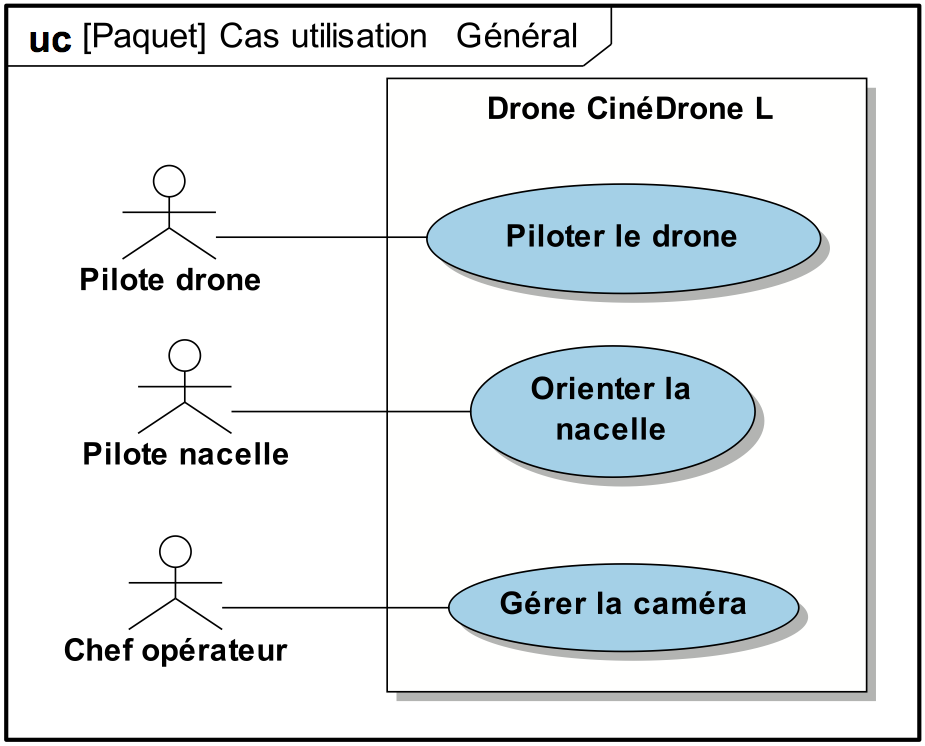
\includegraphics[width=.8\textwidth]{png/PNG/SysML_Drone_Uc}
\end{center}
\end{minipage} \hfill
\begin{minipage}[c]{.45\linewidth}
\begin{center}
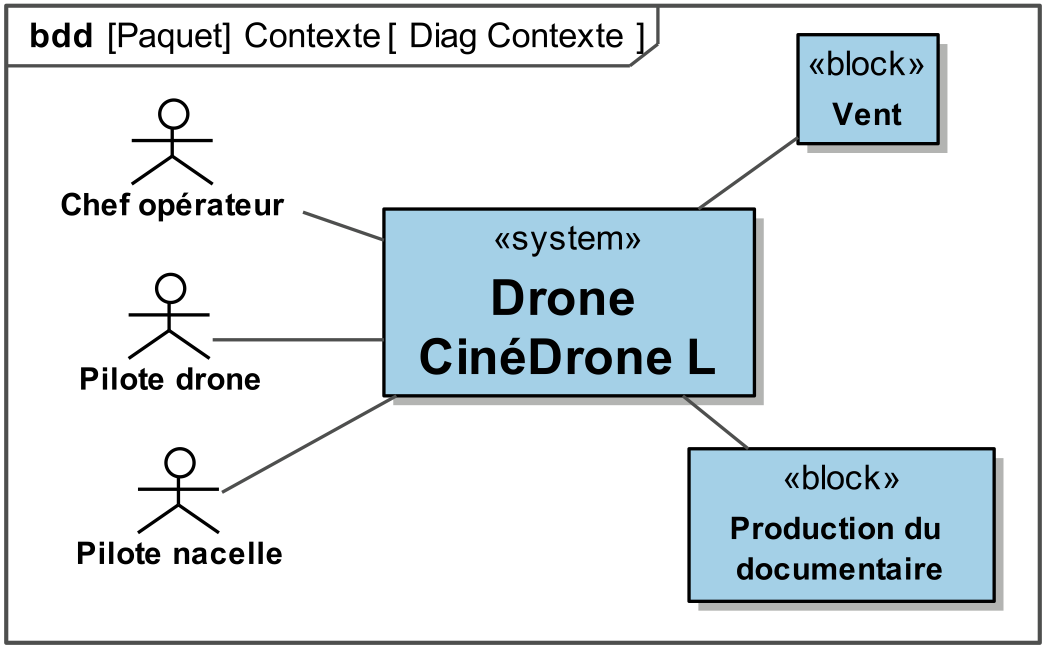
\includegraphics[width=.8\textwidth]{png/PNG/SysML_Drone_Contexte}
\end{center}
\end{minipage}

\end{exemple}


\subsubsection{Diagramme de séquence}

\begin{defi}
\textbf{Diagramme de séquence -- \textit{Sequence Diagram -- seq}}

L’objectif de ce diagramme est de décrire les interactions existant entre plusieurs entités,
celles-ci pouvant être des acteurs, le système ou ses sous-systèmes. Le diagramme ne montre
donc que l’enchaînement séquentiel des différentes interactions.

Un diagramme de séquence est rattaché à un cas d’utilisation et décrit ce dernier en entier
ou en partie, ce qui correspond à un scénario de fonctionnement possible, défini dans un
cadre précis : il peut donc aboutir tout aussi bien à des évolutions positives (fonctionnement
normal) ou négatives (gestion des problèmes), en particulier dans la phase de démarrage
avant le fonctionnement normal.
\end{defi}

\begin{center}
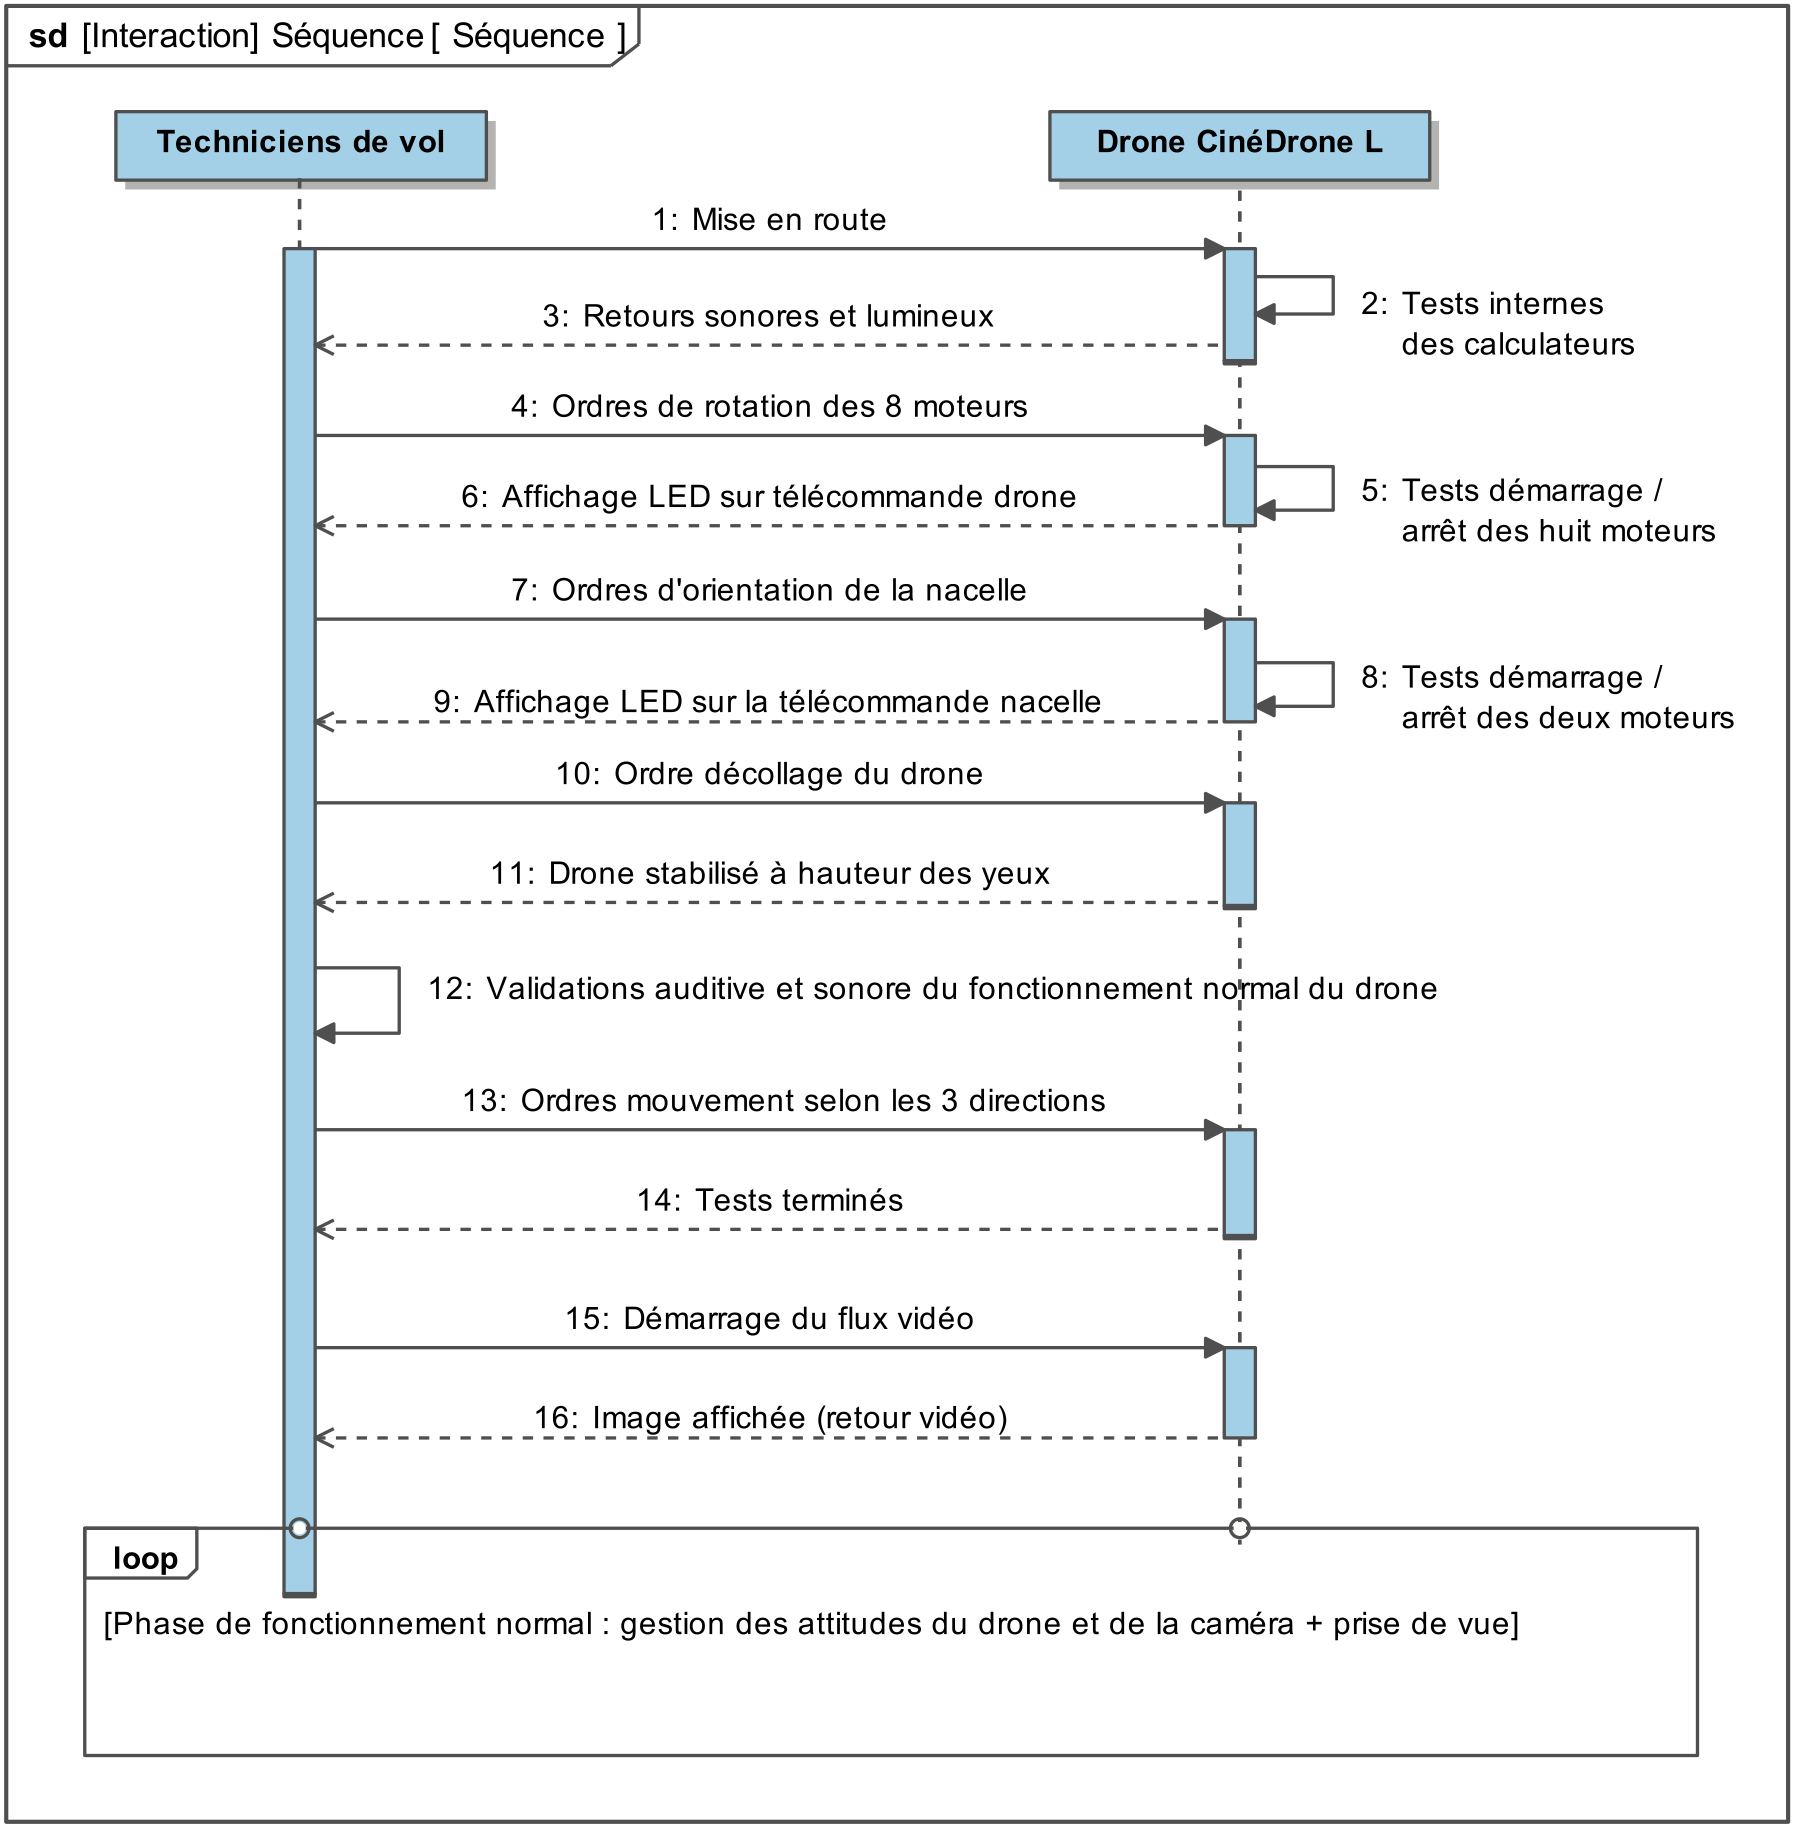
\includegraphics[width=.5\textwidth]{png/PNG/SysML_Drone_Seq}
\end{center}



\subsubsection{Diagramme d'états}
\begin{defi}
\textbf{Diagramme d'états -- \textit{State Machine Diagram - stm}}

Le diagramme d’états est rattaché à un bloc qui peut être le système, un sous-système
ou un composant. Le comportement décrit par ce type de diagramme sert à montrer les
différents états pris par le bloc en fonction des évènements qui lui arrivent.

Un état représente une situation d’une durée finie durant laquelle un système exécute une
activité, satisfait à une certaine condition ou bien est en attente d’un événement. Le passage
d’un état à un autre se fait en franchissant une transition.

\end{defi}

\begin{exemple}
\begin{center}
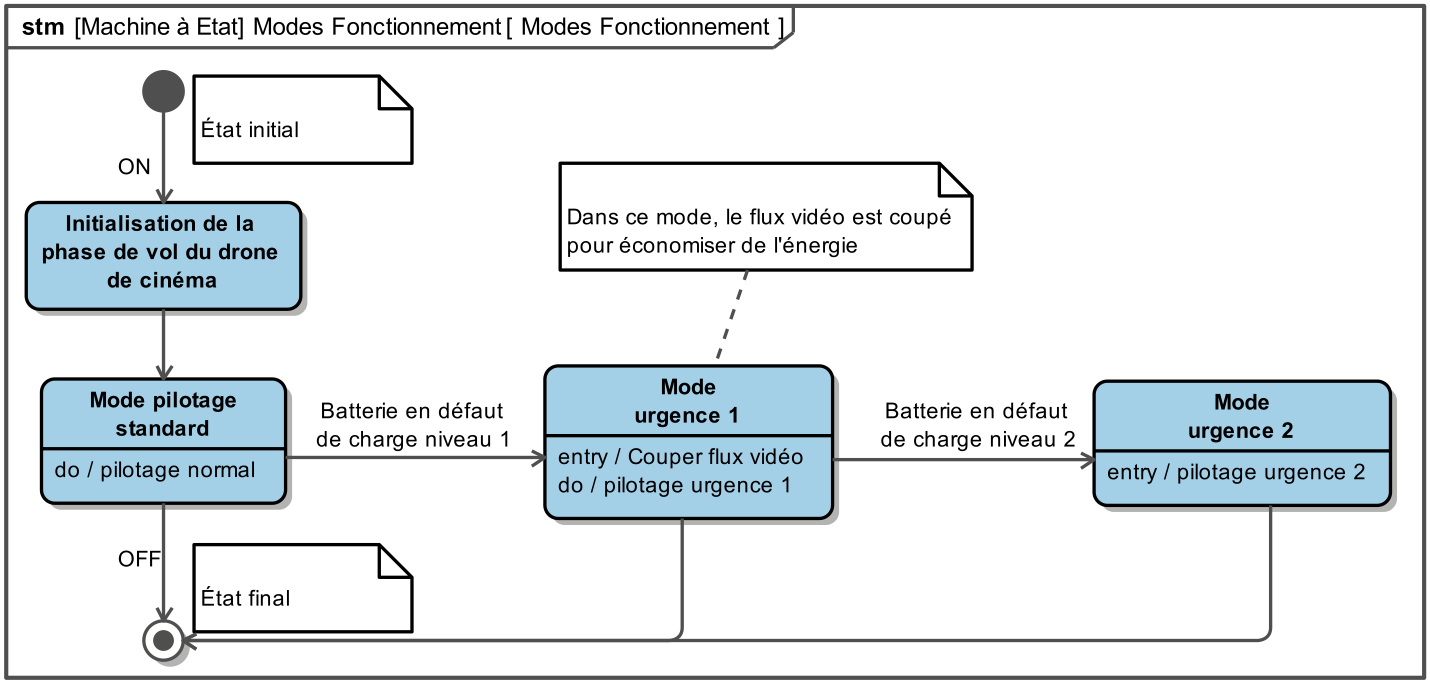
\includegraphics[width=.9\textwidth]{png/PNG/SysML_Drone_Stm}
\end{center}
\end{exemple}

\subsubsection{Diagramme d'activité}

\begin{defi}
\textbf{Diagramme d'activité -- \textit{Activity Diagram -- act}}

Ce diagramme permet de représenter le déroulement d’un processus sous la forme d’une
activité correspondant à une décomposition séquentielle d’actions, aussi appelées tâches.

Dans sa forme la plus restreinte, ce diagramme représente un algorigramme, c’est-à-dire
un flux de contrôle (ce flux n’a rien à voir avec ceux présents dans le diagramme de blocs
internes : il ne faut donc pas les confondre).
\end{defi}

\begin{exemple}

\begin{minipage}[c]{.55\linewidth}
\begin{center}
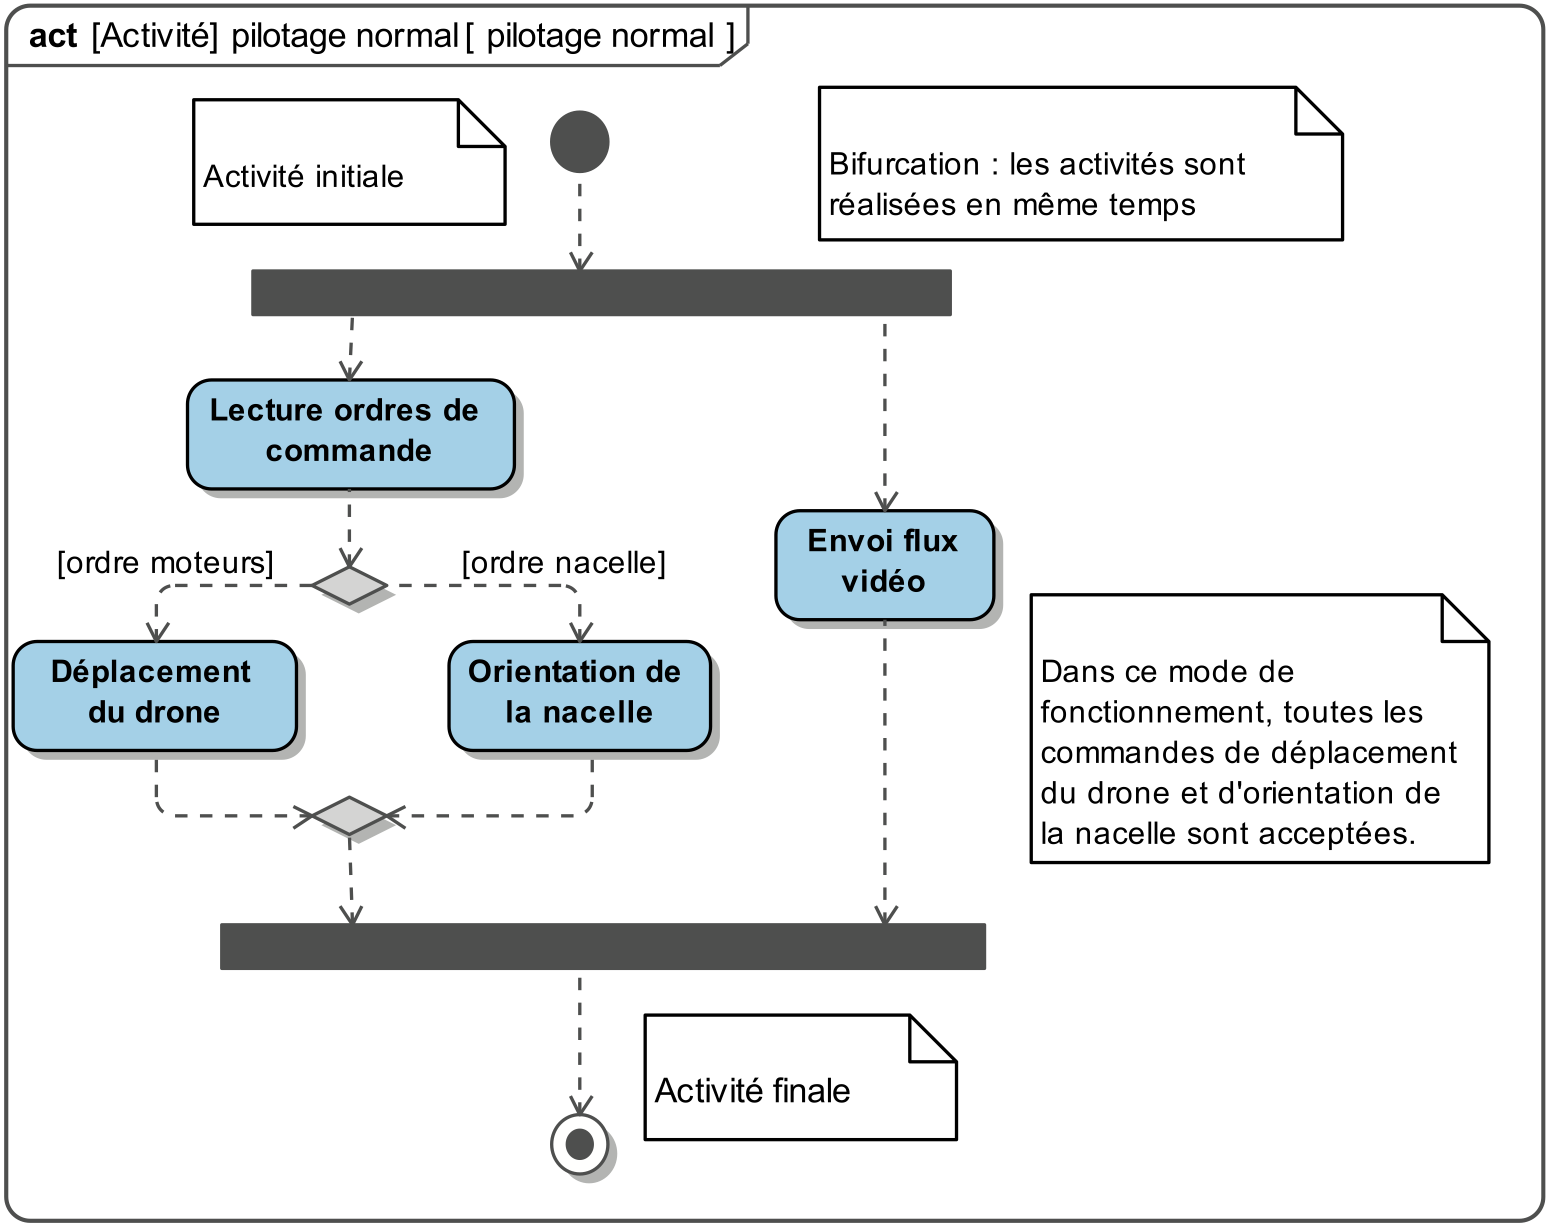
\includegraphics[height=6cm]{png/PNG/SysML_Drone_Act_Normal}
\end{center}
\end{minipage} \hfill
\begin{minipage}[c]{.4\linewidth}
\begin{center}
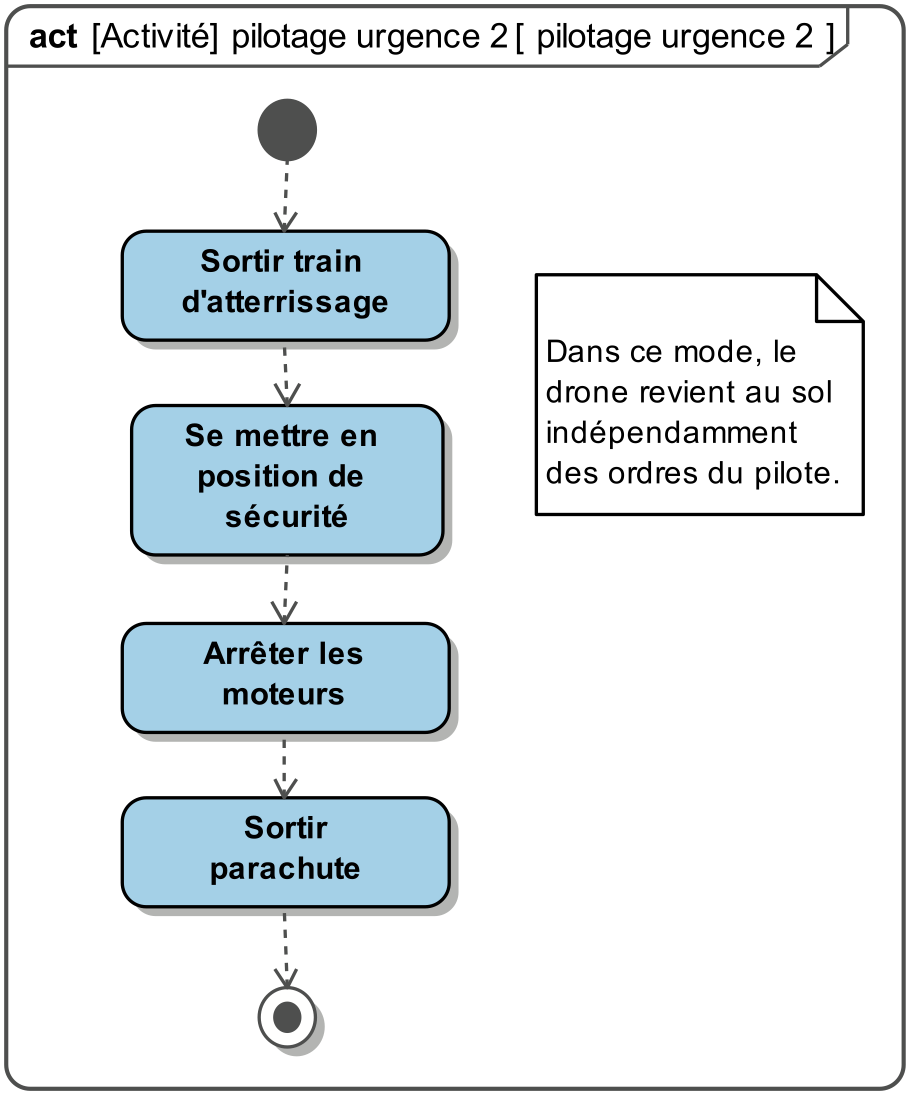
\includegraphics[height=6cm]{png/PNG/SysML_Drone_Act_Urgence2}
\end{center}
\end{minipage}
\end{exemple}
%\begin{center}
%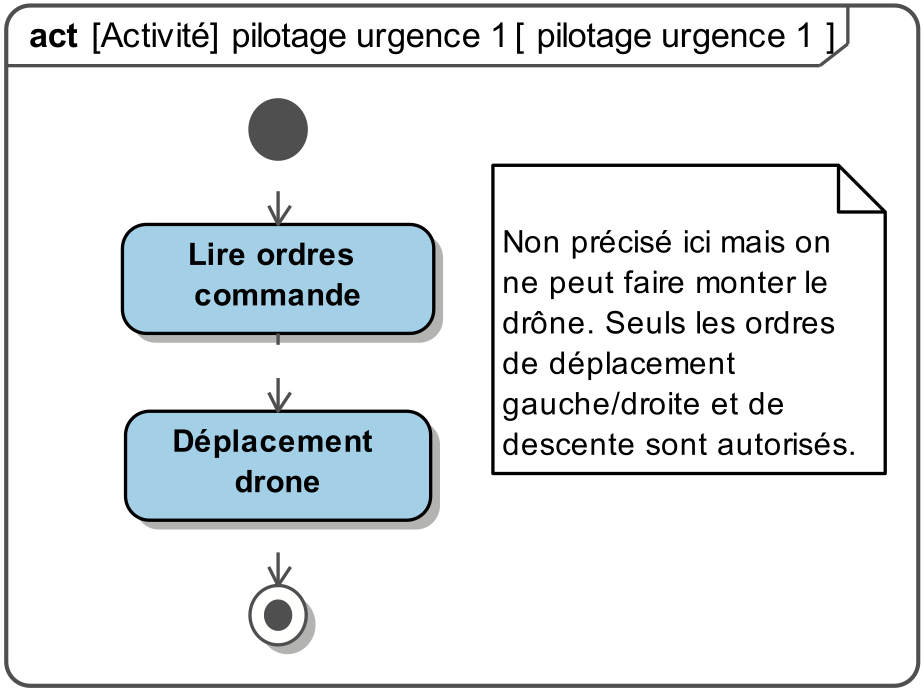
\includegraphics[width=.5\textwidth]{png/PNG/SysML_Drone_Act_Urgence1}
%\end{center}





\subsection{Diagrammes sutructurels}
\subsubsection{Diagramme de définition des blocs}
\begin{defi}
\textbf{Diagramme de définition des blocs -- \textit{Block Definition Diagram - bdd}}
L’objectif de ce diagramme est de décrire le système via des blocs (blocks dans le langage
SysML) et représentant des éléments matériels (cas le plus fréquent) mais également des
entités abstraites (regroupement logique d’éléments) ou des logiciels.

Ce diagramme représente les caractéristiques principales de chaque bloc ainsi que les liens
entre eux : il permet donc une modélisation de l’architecture du système.

\end{defi}

\begin{exemple}
\begin{center}
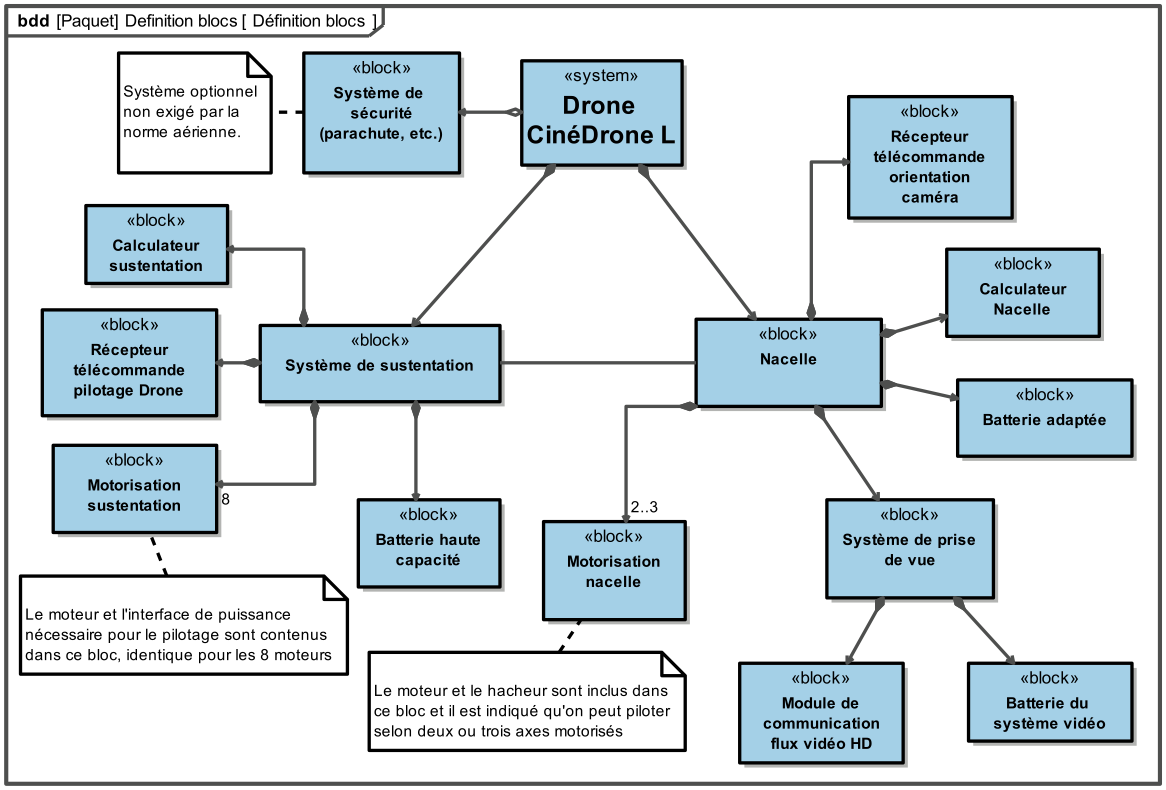
\includegraphics[width=.5\textwidth]{png/PNG/SysML_Drone_Bdd}
\end{center}
\end{exemple}

\subsubsection{Diagramme de blocs internes}

\begin{defi}
\textbf{Diagramme de blocs internes -- \textit{Internal Block Diagram -- ibd}}

Le diagramme de blocs internes est rattaché à un bloc issu du diagramme de définition de
blocs, le cadre du diagramme représentant la frontière d’un bloc.

Le diagramme de définition de blocs introduit la notion fondamentale de « port » qui
correspond à un point d’interaction avec l’extérieur du bloc.

Les connecteurs (traits) entre les ports indiquent soit les associations soit les flux de matière,
d’énergie et d’information entre les différents blocs.

\end{defi}
 
\begin{exemple}
\begin{center}
\includegraphics[width=.9\textwidth]{png/PNG/SysML_Drone_ibd}
\end{center}
\end{exemple}

\subsubsection{Diagramme de paramétriques}
\begin{defi}
\textbf{Diagramme paramétrique -- \textit{Parametric Diagram -- par}}

Ce diagramme est une extension du diagramme de définition de blocs. Il partage donc les mêmes éléments graphiques.

Il présente la particularité de pouvoir connecter entre elles des contraintes ajoutées au
diagramme de blocs par le biais d’un bloc particulier, dit « de contraintes » (constraint block)
qui contient des paramètres et une relation, en général mathématique, les reliant.

\end{defi}

\begin{center}
\textit{Diagramme tiré du tutoriel SusML de l'OMG}

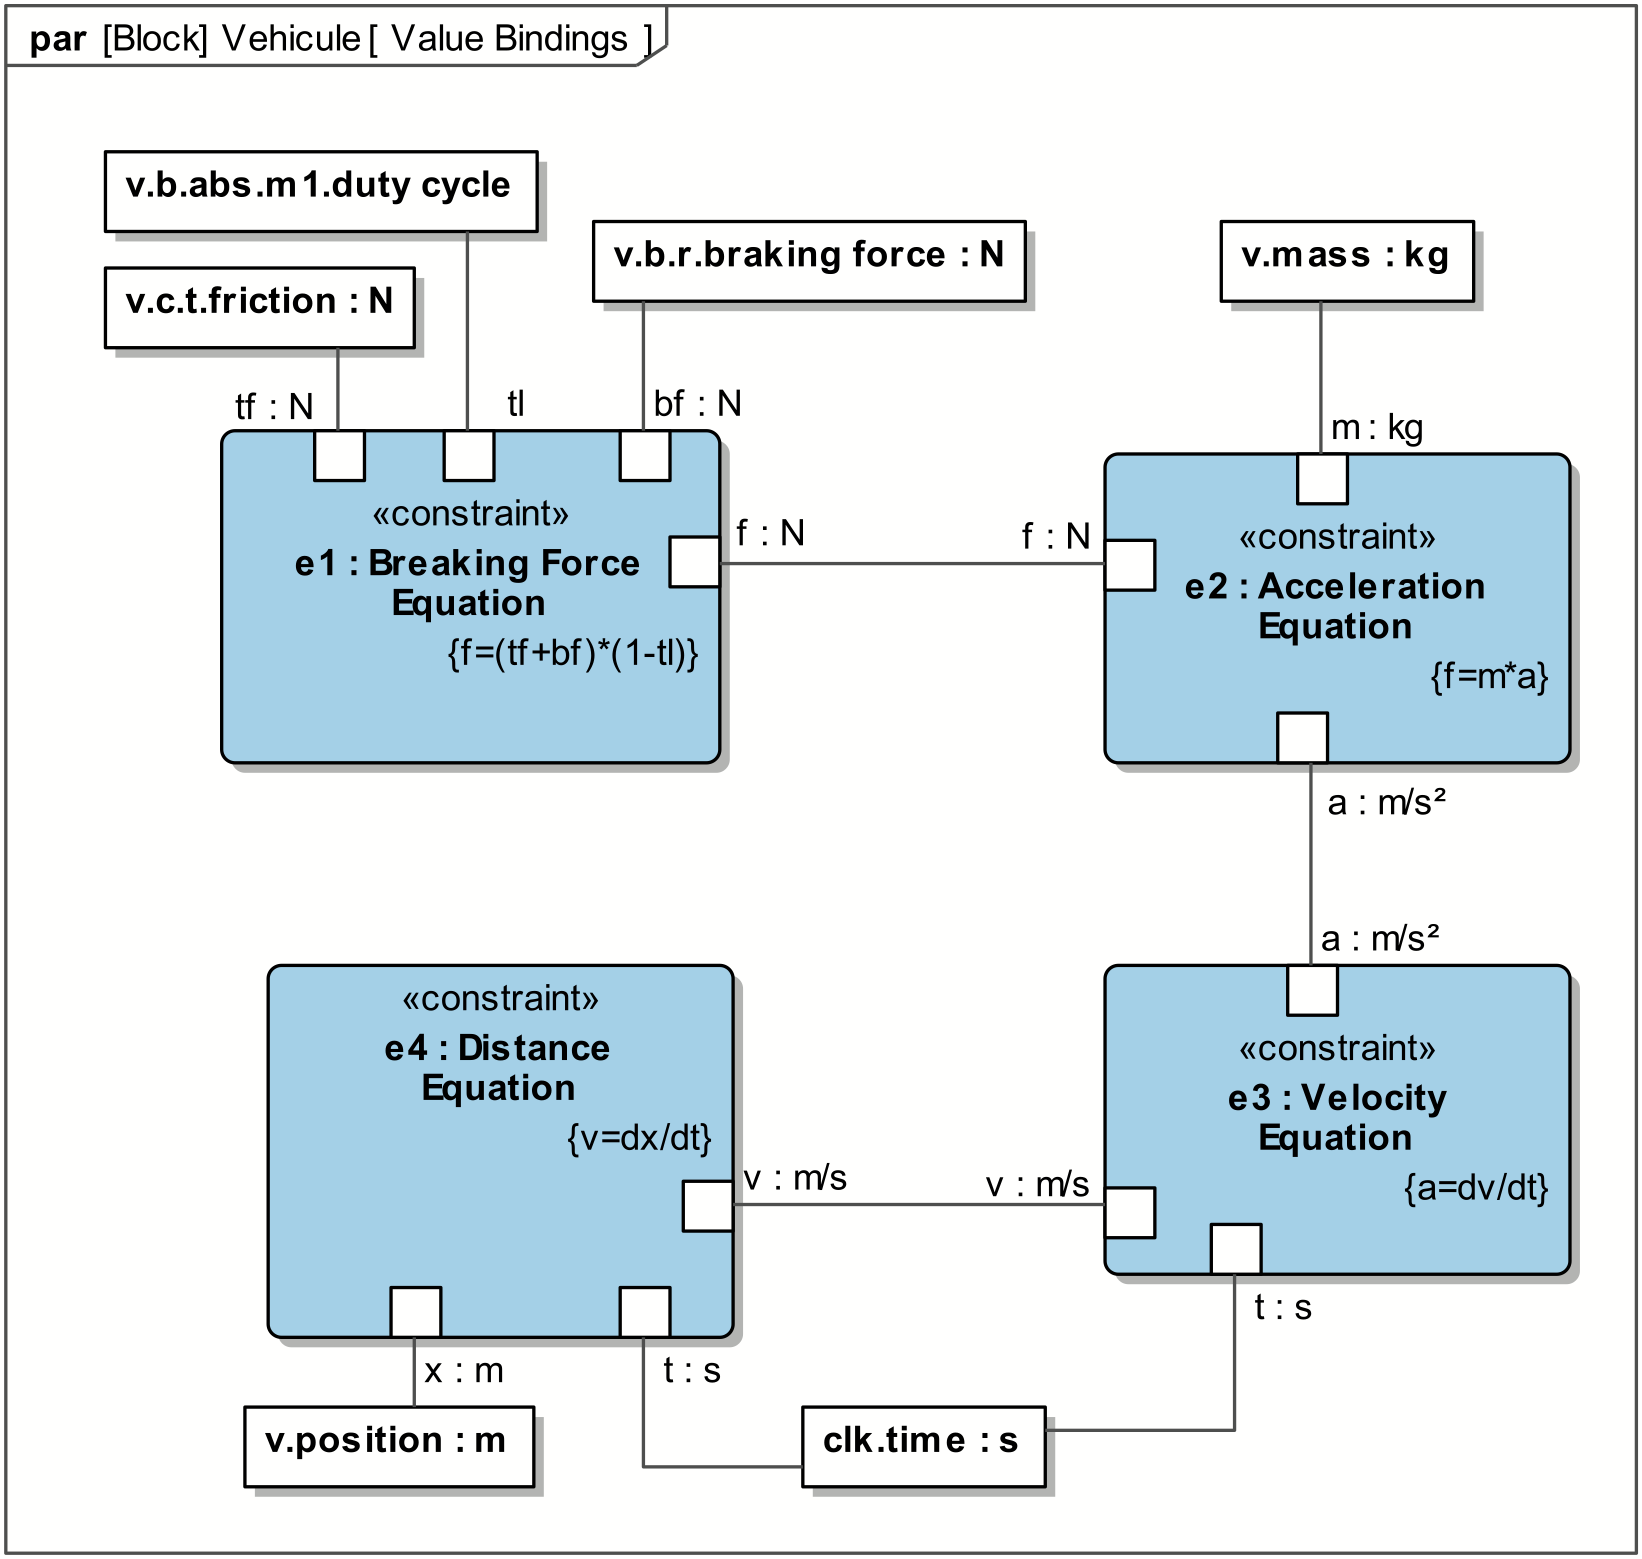
\includegraphics[width=.5\textwidth]{png/PNG/SysML_Drone_Par}
\end{center}
\subsubsection{Diagramme de paquetages}
\begin{defi}
\textbf{Diagramme de paquetages -- \textit{Package Diagram -- pkg}}

L’objectif de ce diagramme est de créer des « macros-associations » de concepts ou d’éléments
afin de relier différentes parties d’un même modèle.

Ce diagramme n’apparaît pas explicitement dans le programme des CPGE : il est donc
donné uniquement à titre d’information.
\end{defi}

\section{Architecture fonctionnelles des systèmes}

\subsection{Chaîne fonctionnelle}
L'avantage de la modélisation SysML est la liberté que le concepteur peut avoir pour décrire un système. L'inconvénient pour un élève en phase d'analyse d'un système est qu'il ne sache pas par quel angle appréhender le système. 


La chaîne fonctionnelle permet de fournir une première grille de lecture pour analyser un système complexe. Elle ne peut pas être la solution pour décrire parfaitement tous les systèmes, mais elle doit être un outil permettant de faire un bilan des macro fonctions qu'il est possible de réaliser. 

\begin{center}
\includegraphics[width=\textwidth]{png/chaine_fonc}
\end{center}

Chacune des fonctions peut être présente où absente sur le système. Dans le cas où la fonction est présente, elle peut être assuré par un ou plusieurs composants. 

\begin{defi}
\textbf{Lien d'information}

Un lien d'information véhicule une information de type électrique (en $V$).

\textbf{Lien de puissance (ou d'énergie)}

Un lien de puissance véhicule une grandeur de type \textbf{effort} et une grandeur de type \textbf{flux}. Le produit de ces deux grandeurs est une puissance.

\end{defi}

\begin{exemple}
\begin{center}
\begin{tabular}{|l|l|l|}
\hline
\textbf{Domaine} & \textbf{Effort} & \textbf{Flux} \\
\hline
\hline
Électrotechnique & Tension ($U$ en $V$) & Courant ($I$ en $A$) \\
\hline
Mécanique de translation & Force ($F$ en $N$) & Vitesse ($V$ en $m/s$) \\
\hline
Mécanique de rotation & Couple ($C$ en $Nm$) & Fréquence de rotation ($\omega$ en $rad/s$) \\
\hline
Hydraulique -- Pneumatique & Pression ($P$ en $Pa$) & Débit volumique ($q$ en $m^3/s$)\\
\hline
Thermique & Température ($T$ en $\textdegree C$) & Flux d'entropie ($Q_S$ en $W/\textdegree C$)\\
\hline
\end{tabular}
\end{center}
\end{exemple}

\begin{exemple}
\textit{Chaîne fonctionnelle d'un véhicule}

\begin{center}
\includegraphics[width=\textwidth]{png/chaine_fonc_ex}
\end{center}
\end{exemple}

\begin{thebibliography}{2}
\bibitem{cc_ex1}{Concept car Peugeot EX1. \url{http://www.peugeot.fr/media/showrooms/showroom-peugeot-ex1-concept-car-kppv3/medias/img/extergrand.jpg}.}
\bibitem{norme}{Norme NF EN 1325-1 (Anciennement NF X50-150), Vocabulaire du Management de la Valeur,de l'Analyse de la Valeur et de l'Analyse Fonctionnelle. Partie 1 : Analyse de la Valeur et de l'Analyse Fonctionnelle.}
\bibitem{roques}{Pascal Roques, SysML par l'exemple -- Un langage de modélisation pour systèmes complexes. Éditions Eyrolles, 2009.}
\bibitem{debout}{Pierre Debout, SII -- Analyse Externe des systèmes.}
\bibitem{sii}{A. Caignot, V. Crespel, M. Dérumeaux, C. Garreau, P. Kaszynski, B. Martin \& S. Roux. Sciences Industrielles de l'Ingénieur -- MPSI -- PCSI -- PTSI.}

\bibitem{oled}{\url{http://reload4btech.blogspot.fr/2012/06/philips-flexible-oled-fluid-smartphone.html}}
\bibitem{pont}{\url{http://projets-architecte-urbanisme.fr/images-archi/2013/03/pont-bacalan-chaban-delmas.jpg}}
\bibitem{vibram}{\url{http://www.vibramfivefingers.it/images/products/FFSKSAAYM.jpg}}
\bibitem{magsurf}{\url{http://www.univ-paris-diderot.fr/sc/site.php?bc=accueil&np=pageActu&ref=3658}}
\bibitem{segway}{\url{http://www.segway.fr/particuliers/gyropodes/x2.htm}}
\bibitem{audi}{\url{http://www.nerdpix.com/design/un-velo-electrique-vraiment-moderne/}}
\bibitem{embouti}{\url{http://www.esi-group.com/corporate/news-media/press-releases/2007-french-pr/archives/esi-group-annonce-pam-tfa-pour-catia-v5-une-nouvelle-solution-pam-stamp}}
\bibitem{fao}{\url{http://www.directindustry.fr/prod/sprut-technology-inc/logiciels-de-simulation-d-usinage-cnc-66031-742439.html}}
\bibitem{ef}{\url{http://www.mscsoftware.com/fr/application/simulation-numerique-multidisciplinaire}}
\bibitem{scilab}{\url{http://www.demosciences.fr/projets/scilab-xcos/utilisation/pour-aller-plus-loin}}
\bibitem{wafer}{\url{http://www.erenumerique.fr/technologie_dessine_moi_un_capteur_d_image-article-4943-2.html}}
\bibitem{u5x}{\url{http://www.machine-outil.info/t325-bridage-usinage-serrage-usinage/a4590-un-etau-specifique-pour-machine-5-axes-chez-norelem.html}}
\bibitem{injection}{\url{http://french.plastic-injectionmould.com/china-oem_lkm_pretreat_single_cavity_custom_plastic_injection_molding_for_pc_abs_plastic_chair-212008.html}}
\bibitem{satellite}{\url{http://www.astrium-geo.com/fr/2834-decembre-2011-spot-6-couplage-de-linstrument-a-la-plate-forme}}

\end{thebibliography}

\end{document}